\chapter{Experiments}
\label{ch:appendix-experiments}

In this chapter, we present additional experiments, further qualitative examples
as well as details regarding training and evaluation.

\section{Training Details}

For training, we use stochastic gradient descent with momentum and weight decay.
The initial learning rate was experimentally determined to be $\gamma^{(0)} = 10^{-6}$
for most experiments; for experiments involving signed distance functions the initial
learning rate might be slightly slower, \eg $\gamma^{(0)} = 5\cdot10^{-7}$ -- 
on the 2D dataset we even reduced it to $\gamma^{(0)} = 5\cdot10^{-8}$ when training
signed distance functions only.
It is then reduced every $T_{\gamma} = 500$ iterations using $\alpha_{\gamma} = 0.95$.
The minimum learning rate $\gamma_{\min} = 10^{-15}$ is usually only reached
for training the shape prior, which involves significantly more epochs than
training the inference models. We usually use a momentum of $\beta^{(0)} = 0.5$
and increase it every $T_{\beta} = T_{\alpha} = 500$ iterations with a factor
$\alpha_{\beta} = 1.025$ until $\beta_{\max} = 0.9$ is reached. In 2D,
because training is easier, we increase the momentum term using
$\alpha_{\beta} = 1.05$ instead. For weight decay,
we usually use a weight of $\kappa = 10^{-6}$. We trained the shape prior to
up to $250$ epochs; and inference models usually up to $25$ epochs -- except
on KITTI \cite{GeigerLenzUrtasun:2012,GeigerLenzStillerUrtasun:2013}
where significantly more epochs are used as the dataset is very small.
We always present results corresponding to a model trained for the optimal
number of iterations determined using early stopping.
We found that weight decay has negligible influence on the obtained performance,
but slightly helps training. Additionally, the initial learning
rate has a significant effect when chosen
too large -- in the extreme case, training diverges in the first few iterations.
Using a momentum term helps in all cases and gradually reducing the learning
rate is necessary to obtain good results. We always use Xavier initialization
\cite{GlorotBengio:2010}. We also experimented with
alternative optimization algorithms, \eg ADAM \cite{KingmaBa:2014}, but
found standard stochastic gradient descent to work most reliably.

\section{Evaluation}
\label{sec:appendix-experiments-evaluation}

We claimed that the negative log-likelihood is unsuited for evaluation
partly because it favors ``unsure'' predictions, \ie occupancy probabilities
close to $0.5$ over very certain predictions with few mistakes. The following
example is intended to illustrate this:

\begin{example}
  We consider a $R$-dimensional binary volume representing a shape. Let 
  $y \in [0,1]^R$ the predicted shape; let $y^* \in \{0,1\}^R$ be the true shape.
  Assuming $y$ fits $y^*$ perfectly, the negative log-likelihood is zero.
  Flipping the prediction of one $y_i = 1$ to $y_i \approx 0.0001$ (due to
  numerical stability) changes the negative log likelihood to $\sim 9.21$.
  Then, we can set
  $\frac{-\ln 0.0001}{- \ln 0.5} \approx \frac{9.21}{0.693} \approx 9.966$
  of $y^*$'s occupied voxels to $0.5$ and the negative log-likelihood will not exceed $9.21$.
  In practice, this means that an ``unsure'' model predicting an occupancy probability
  of $0.5$ for many pixels will have a lower negative log-likelihood
  than a nearly perfect prediction with few but very certain mistakes.
\end{example}

\section{2D Example}
\label{sec:appendix-experiments-2d}

% TODO auto-encoders or auto-encoder
We originally developed the 2D dataset to understand how probabilistic PCA (\PPCA) and variational
auto-encoders (\VAEs) can learn shape priors; and to provide a proof of concept
that the methods for shape inference introduced in Chapter \ref{ch:shape-inference}
as well as in Appendix \ref{ch:appendix-shape-inference}
are applicable. We also intend to present a short quantitative comparison to
identify well-performing approaches in order to proceed to the 3D datasets as 
well as KITTI.

% TODO nicer tables
\begin{table}
  \centering
  {\footnotesize
  \renewcommand{\arraystretch}{1.1}
  \begin{tabularx}{\textwidth}{| X | c | c | c |}
    \hline
    & \Rect\easy & \Rect\moderate & \Rect\hard\\\hline
    Training Size (Prior/Inference) & \multicolumn{3}{c|}{$10000/10000$}\\\hline
    Validation Size & \multicolumn{3}{c|}{$1000$}\\\hline
    Resolution $H \times W$ & \multicolumn{3}{c|}{$32 \times 32$}\\\hline
    Resolution $2u$ & $64$ & \multicolumn{2}{c|}{$32$}\\\hline
    Noise $\theta_{\text{hit}}$ & $1$ & $0.75$ & $0.75$\\\hline
    Noise $\theta_{\text{ignore}}$ & $0$ & $0$ & $0.1$\\\hline
    Observed Voxels (Inference Training Set) & $1.79\%$ & $1.09\%$ & $0.97\%$\\\hline
    Free Space Voxels (Inference Training Set) & $13.63\%$ & $10.99\%$ & $16.59\%$\\\hline
    Occupied Voxels (Inference Training Set) & $29.6\%$ & $29.57\%$ & $29.31\%$\\\hline
  \end{tabularx}
  }
  \vskip 6px
  % TODO short caption
  \caption{Overview of the generated datasets. We created datasets of three
  difficulties, \easy, \moderate and \hard, which refer to increased noise
  and less observations. Additionally, we report statistics such as the
  percentage of observed voxels, free space voxels and occupied voxels
  (of the ground truth shapes) over the training set used for shape inference.}
  \label{table:experiments-2d-datasets}
\end{table}

For all experiments regarding
shape completion, we constructed three datasets of varying difficulties:
\easy, \hard and \moderate with details in Table \ref{table:experiments-2d-datasets}.
In all three cases, we always use partial free space
as this will also be the case on KITTI.
With rising difficulty, less observations are provided and the underlying
noise increases. The \hard case is supposed to represent real conditions
as found on KITTI.

The experimental setup follows Chapter \ref{ch:experiments}. Additionally,
\PPCA was implemented using SciPy's sparse SVD implementation\footnote{
  \url{https://docs.scipy.org/doc/scipy/reference/generated/scipy.sparse.linalg.svds.html}.
} and $\sigma^2$ from Definition \ref{def:shape-prior-ppca} was approximated
using the first $\rho \cdot HW$ eigenvalues of the data matrix; here, $\rho$
is the fraction of pixels occupied over the whole training set. The 
$Q$ largest eigenvalues are chosen to determine the projection $U$ and the
remaining ones are used to compute $\sigma^2$. We found this heuristic to work
well in both 2D and 3D. In the 2D case, $\rho \approx 0.297$ and for $H \times W = 32 \times 32$,
we have $\rho HW \approx 302$.

\subsection{Shape Prior}
% TODO goal: understand how shapes can be modeled
% - how large should code size be
% - how large should the network be
% - what reconstruction error can be expected
% - how much data do we need

First, we want to understand how well \PPCA and \VAEs can learn a shape prior
-- especially regarding the latent space, \eg its dimensionality and the
quality of random samples.
For \VAEs we are additionally interested in the two introduced representations
-- occupancy and signed distance functions.

\subsubsection{Probabilistic PCA}

\begin{figure}
  \centering
  % http://pgfplots.sourceforge.net/gallery.html
  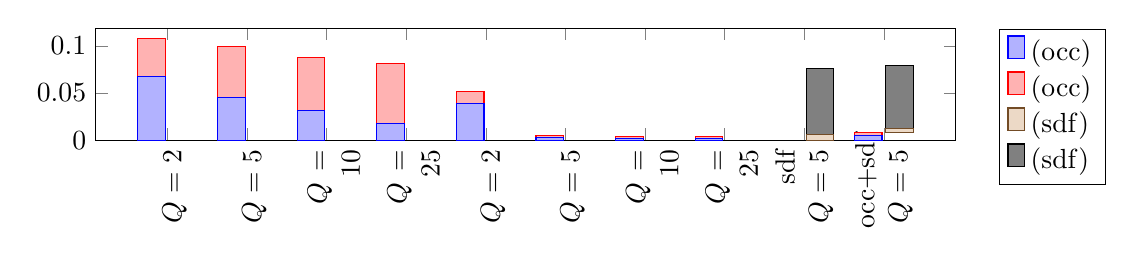
\begin{tikzpicture}
    \begin{axis}[
        ybar stacked,
        % https://tex.stackexchange.com/questions/119887/remove-the-scientific-notation-which-is-unreasonable
        yticklabel style={
          /pgf/number format/fixed,
          /pgf/number format/precision=5
        },
        scaled y ticks=false,
        legend style={
          at={(1.05,1)},
          anchor=north west,
        },
        % https://tex.stackexchange.com/questions/48620/pgfplots-alignment-and-size-of-math-in-legend
        legend cell align=left,
        % https://tex.stackexchange.com/questions/135595/how-to-correct-problem-with-ybar-plot-bad-axis-and-too-many-labels-in-x-axis
        xtick={
          1, 2, 3, 4,
          5, 6, 7, 8,
          9, 10
        },
        xticklabels={
          \PPCA\\$Q = 2$, \PPCA\\$Q = 5$, \PPCA\\$Q = 10$, \PPCA\\$Q = 25$,
          \VAE\\$Q = 2$, \VAE\\$Q = 5$, \VAE\\$Q = 10$, \VAE\\$Q = 25$,
          \VAE sdf\\$Q = 5$, \VAE occ+sdf\\$Q = 5$
        },
        x tick label style={text width=1cm,align=right},
        ymin=0,
        height=3cm,
        width=12.5cm,
        % https://tex.stackexchange.com/questions/271027/pgfplots-how-to-rotate-extra-x-tick-labels
        x tick label style={
          rotate=90,
          anchor=east,
        },
      ]
      
      % AbsThr
      \addplot +[bar shift=-.2cm] coordinates {
        (1, 0.06709765625)
        (2, 0.0449326171875)
        (3, 0.0312314453125)
        (4, 0.0177939453125)
        (5, 0.03853159)
        (6, 0.00318352)
        (7, 0.00182621)
        (8, 0.00181555)
        (9, 0)
        (10, 0.00499229)
      };
      \addlegendentry{\AbsThr (occ)}
      % Abs
      \addplot +[bar shift=-.2cm] coordinates {
        (1, 0.0404) % 0.107466870529)
        (2, 0.0542) % 0.0973753175757)
        (3, 0.05637) % 0.0876120861329)
        (4, 0.0634) % 0.0711613035139)
        (5, 0.01271) % 0.05121126)
        (6, 0.001974) % 0.00515391)
        (7, 0.001784) % 0.00361275)
        (8, 0.00185) % 0.00366516)
        (9, 0)
        (10, 0.002778) % 0.00777563)
      };
      \addlegendentry{\Abs (occ)}
      
      \resettenstackedplots
      
      %
      \addplot +[bar shift=.2cm]coordinates {
        (1, 0)
        (2, 0)
        (3, 0)
        (4, 0)
        (5, 0)
        (6, 0)
        (7, 0)
        (8, 0)
        (9, 0.00623527)
        (10, 0.00514245)
      };
      \addlegendentry{\AbsThr (sdf)}
      %
      \addplot +[bar shift=.2cm] coordinates {
        (1, 0)
        (2, 0)
        (3, 0)
        (4, 0)
        (5, 0)
        (6, 0)
        (7, 0)
        (8, 0)
        (9, 0.070219) % 0.07644901)
        (10, 0.06591859) % 0.07105859)
      };
      \addlegendentry{\Abs (sdf)}
    \end{axis}
  \end{tikzpicture}
  % TODO short caption
  \caption{Absolute error \Abs and its thresholded pendant
  \AbsThr, \ie the absolute error after thresholding the predicted shapes,
  for \PPCA and \VAE with different size $Q \in \{2,5,10,25\}$ of the
  latent space. For \VAE we additionally compare the different representations,
  \ie occupancy (occ) and signed distance functions (sdf). For \PPCA we only
  report results on occupancy. Note that
  for \VAEs and occupancy, \Abs and \AbsThr are usually very close together.
  In each case, the bars on the left represent result son occupancy (if applicable);
  while the bars on the right correspond to results on signed distance functions
  (if applicable).}
  \label{fig:experiments-2d-ppca}
\end{figure}

\begin{figure}
  \centering
  \begin{tikzpicture}
    \node at (0,2.5) {$Q = 2$};
    \node at (0,0) {\includegraphics[width=3cm]{experiments/2d/ppca_occ/easy_2/results}};
    \node at (0,-3.25) {\includegraphics[width=3cm]{experiments/2d/ppca_occ/easy_2/random2}};
    \draw[-,dashed] (1.625, -4.75) -- (1.625, 2.5);
    
    \node at (3.25,2.5) {$Q = 5$};
    \node at (3.25,0) {\includegraphics[width=3cm]{experiments/2d/ppca_occ/easy_5/results}};
    \node at (3.25,-3.25) {\includegraphics[width=3cm]{experiments/2d/ppca_occ/easy_5/random2}};
    \draw[-,dashed] (3.25 + 1.625, -4.75) -- (3.25 + 1.625, 2.5);
    
    \node at (6.5,2.5) {$Q = 10$};
    \node at (6.5,0) {\includegraphics[width=3cm]{experiments/2d/ppca_occ/easy_10/results}};
    \node at (6.5,-3.25) {\includegraphics[width=3cm]{experiments/2d/ppca_occ/easy_10/random2}};
    \draw[-,dashed] (6.55 + 1.625, -4.75) -- (6.5 + 1.625, 2.5);
    
    \node at (9.75,2.5) {$Q = 25$};
    \node at (9.75,0) {\includegraphics[width=3cm]{experiments/2d/ppca_occ/easy_25/results}};
    \node at (9.75,-3.25) {\includegraphics[width=3cm]{experiments/2d/ppca_occ/easy_25/random2}};
    \node at (11.75,-1.1) {\includegraphics[height=6.8cm]{experiments/2d/ppca_occ/colorbar2}};
  \end{tikzpicture}
  % TODO short caption
  \caption{Qualitative results for \PPCA with different sizes $Q \in \{2,5,10,25\}$
  of the latent space. From top to down, we show the input shape,
  the reconstruction, the corresponding error and the thresholded reconstruction.
  The last two rows show random samples. We clipped the visualization
  to $[0, 1]$ for convenience.}
  \label{fig:experiments-2d-ppca-qual}
\end{figure}


In Figure \ref{fig:experiments-2d-ppca}, we first consider \PPCA to learn shape priors
to understand the influence of the size of the latent space, \ie $Q$.
Obviously, increasing $Q$ leads to better reconstruction errors.
As comparison, roughly $29.7$ percentage of
pixels are occupied, \ie predicting all zero would result in an error of
approximately $\Abs = \AbsThr \approx 0.297$.  The corresponding
qualitative results in Figure \ref{fig:experiments-2d-ppca-qual}, for $Q = 2$, show
what \PPCA actually does: it uses principal directions to approximate
its input. Increasing $Q$ allows \PPCA to capture more variation, leading
to better reconstructions but also allowing more variation in random samples.
For shape inference, we require that the latent space holds only ``reasonable''
shapes. Taking this into account $Q = 5$ seems to be
a reasonable trade-off between reconstruction error and appropriate samples.

\subsubsection{Variational Auto Encoder}
\label{sec:experiments-2d-vae-prior}

% TODO coherent colors!
\begin{figure}
  \centering
  \begin{subfigure}[t]{0.48\textwidth}
    \begin{tikzpicture}
      \begin{axis}[
          % https://tex.stackexchange.com/questions/68577/compiling-a-document-with-pgfplots-processing-only-every-x-th-data-point
          %each nth point=100,
          filter discard warning=false,
          unbounded coords=discard,
          % https://tex.stackexchange.com/questions/13816/dimension-too-large-while-plotting-with-pgfplots
          %restrict y to domain=0:0.1,
          %restrict x to domain=0:250000,
          %ymin=0,
          ymax=0.4,
          xmin=0,
          xmax=250000,
          %xticklabel={
          %  \pgfmathparse{\tick/1000}
          %  \pgfmathprintnumber{\pgfmathresult}k
          %},
          xtick={0,50000,100000,150000,200000,250000},
          xticklabels={0,50k,100k,150k,200k,250k},
          xticklabel style={
            /pgf/number format/fixed
          },
          scaled x ticks=false,
          yticklabel style={
            /pgf/number format/fixed
          },
          scaled y ticks=false,
          %x coord trafo/.code={\pgfmathparse{\pgfmathresult/1000}},
          %xticklabel=\pgfmathprintnumber{\tick}k,
          width=7.5cm,
          height=5cm,
          % https://tex.stackexchange.com/questions/48620/pgfplots-alignment-and-size-of-math-in-legend
          legend cell align=left,
        ]
        
        \addplot +[mark=none] table[ignore chars={(,)},col sep=comma] {data/experiments/2d/vae_occ/easy_5/validation_mean.txt};
        \addlegendentry{$\overline{\mu}$ (val)};
        \addplot +[mark=none] table[ignore chars={(,)},col sep=comma] {data/experiments/2d/vae_occ/easy_5/validation_var.txt};
        \addlegendentry{$\exp\left(\frac{1}{2}\overline{l}\right)$ (val)};
        \addplot +[mark=none] table[ignore chars={(,)},col sep=comma] {data/experiments/2d/vae_occ/easy_5/validation_std.txt};
        \addlegendentry{$|1 - \sqrt{\Var[\mu]}|$ (val)};
        \addplot +[mark=none] table[ignore chars={(,)},col sep=comma] {data/experiments/2d/vae_occ/easy_5/validation_abs.txt};
        \addlegendentry{$\Abs$ (val)};
      \end{axis}
    \end{tikzpicture}
  \end{subfigure}
  \begin{subfigure}[t]{0.48\textwidth}
    \begin{tikzpicture}
      \begin{axis}[
          % https://tex.stackexchange.com/questions/68577/compiling-a-document-with-pgfplots-processing-only-every-x-th-data-point
          %each nth point=100,
          filter discard warning=false,
          unbounded coords=discard,
          % https://tex.stackexchange.com/questions/13816/dimension-too-large-while-plotting-with-pgfplots
          %restrict y to domain=0:0.1,
          %restrict x to domain=0:250000,
          %ymin=0,
          ymax=0.5,
          xmin=0,
          xmax=250000,
          %xticklabel={
          %  \pgfmathparse{\tick/1000}
          %  \pgfmathprintnumber{\pgfmathresult}k
          %},
          xtick={0,50000,100000,150000,200000,250000},
          xticklabels={0,50k,100k,150k,200k,250k},
          xticklabel style={
            /pgf/number format/fixed
          },
          scaled x ticks=false,
          yticklabel style={
            /pgf/number format/fixed
          },
          scaled y ticks=false,
          %x coord trafo/.code={\pgfmathparse{\pgfmathresult/1000}},
          %xticklabel=\pgfmathprintnumber{\tick}k,
          width=7.5cm,
          height=5cm,
          % https://tex.stackexchange.com/questions/48620/pgfplots-alignment-and-size-of-math-in-legend
          legend cell align=left,
          legend style={
            anchor=north east,
            at={(0.975,0.75)},
          },
        ]
        
        \addplot +[mark=none] table[ignore chars={(,)},col sep=comma] {data/experiments/2d/vae_occ/easy_25/validation_mean.txt};
        \addlegendentry{$\overline{\mu}$ (val)};
        \addplot +[mark=none] table[ignore chars={(,)},col sep=comma] {data/experiments/2d/vae_occ/easy_25/validation_var.txt};
        \addlegendentry{$\exp\left(\frac{1}{2}\overline{l}\right)$ (val)};
        \addplot +[mark=none] table[ignore chars={(,)},col sep=comma] {data/experiments/2d/vae_occ/easy_25/validation_std.txt};
        \addlegendentry{$|1 - \sqrt{\Var[\mu]}|$ (val)};
        \addplot +[mark=none] table[ignore chars={(,)},col sep=comma] {data/experiments/2d/vae_occ/easy_25/validation_abs.txt};
        \addlegendentry{$\Abs$ (val)};
      \end{axis}
    \end{tikzpicture}
  \end{subfigure}
  % TODO short caption
  \caption{Absolute error \Abs, average $\overline{\mu}$ of the predicted means,
  the corresponding standard deviation $\sqrt{\Var[\mu]}$ and the average
  $\exp(\frac{1}{2}\overline{l})$ of the predicted standard deviations 
  on the validation set for
  \VAEs trained with $Q = 5$ (left) and $Q = 25$ (right). For the actually
  observed standard deviation, we plot its deviation from $0$ for convenience,
  \ie $|1 - \sqrt{\Var[\mu]}|$. We refer to
  Equations \eqref{eq:shape-prior-monitor-mean-mean},
  \eqref{eq:shape-prior-monitor-variance-mean} and \eqref{eq:shape-prior-monitor-mean-variance}
  for details. Note that for $Q = 25$, the actual standard deviation
  collapses to roughly $0.55$ such that $|1 - \sqrt{\Var[\mu]}|$ approaches
  $\sim 0.45$ meaning that the unit Gaussian prior is not met.}
  \label{fig:experiments-2d-vae-occ-5}
\end{figure}

\begin{figure}
  \centering
  \vspace*{-0.5cm}
  \begin{tikzpicture}
    \node at (0, 0){\includegraphics[width=5cm]{experiments/2d/vae_occ/easy_5/results_226000}};
    \node at (0, -4.25){\includegraphics[width=5cm]{experiments/2d/vae_occ/easy_5/random_226000}};    
    \draw[-,dashed] (2.75, -13.25) -- (2.75, 1.5);
    
    \node at (5.5, 0){\includegraphics[width=5cm]{experiments/2d/vae_occ/easy_25/results_245000}};
    \node at (5.5, -4.25){\includegraphics[width=5cm]{experiments/2d/vae_occ/easy_25/random_245000}};
   
    \node at (0, 2.25) {\begin{tabular}{c}$Q = 5$\\occupancy\end{tabular}};
    \node at (5.5, 2.25) {\begin{tabular}{c}$Q = 25$\\occupancy\end{tabular}};
    
    \node at (8.5,-4.25) {
      \includegraphics[height=5.5cm]{experiments/2d/ppca_occ/colorbar2}
    };
    
    \draw[-,dashed] (-2.75,-7) -- (8.5,-7);
    
    \node at (0, -9.75){
      \includegraphics[width=5cm]{experiments/2d/vae_occ_sdf/easy_5_long/results_0}
    };    
    \draw[-,dashed] (2.75, -2.75) -- (2.75, 3);
    
    \node at (5.5, -9.75){
      \includegraphics[width=5cm]{experiments/2d/vae_occ_sdf/easy_5_long/results_1}
    };
    \node at (8.5,-9.75) {\includegraphics[height=5.5cm]{experiments/2d/vae_occ_sdf/easy_5_long/colorbar_1}};
   
    \node at (0, -13.25) {\begin{tabular}{c}$Q = 5$\\occupancy\end{tabular}};
    \node at (5.5, -13.25) {\begin{tabular}{c}$Q = 5$\\signed distance functions\end{tabular}};
    
    \node[rotate=90] at (-3.5, -3) {\begin{tabular}{c}predicting occupancy only\end{tabular}};
    \node[rotate=90] at (-3.5, -9.75) {\begin{tabular}{c}predicting occupancy and\\signed distance functions\end{tabular}};
  \end{tikzpicture}
  \vskip 6px
  
  % TODO short caption
  \caption{A comparison of random samples for \VAE shape rpiors using $Q = 5$
  and $Q = 25$ for occupancy only
  (top) and $Q = 5$ for occupancy and signed distance functions (bottom).
  In the former case, we show reconstructions of five samples for $Q = 5$
  and $Q = 25$, respectively, illustrating target shape in the first row,
  followed by the prediction and its error. Below we show $25$ random samples.
  For the latter case, we show the target shapes in the first row,
  the reconstruction and the corresponding error
  in the next two rows and, finally, two rows of random samples.}
  \label{fig:experiments-2d-vae-occ-random}
\end{figure}


Next, we consider the \VAE equivalent using occupancy as shape representation.
First of all, we discuss training; Figure \ref{fig:experiments-2d-vae-occ-5}
shows absolute error \Abs on the validation set for $Q = 5$.
We additionally monitor the predicted means through $\Var[\mu]$ and $\overline{\mu}$
as well as the predicted standard deviations, \ie $\exp(\frac{1}{2}\overline{l})$.
As can be seen, network training seems to stagnate after around $100k$
iterations according to the reconstruction error.
However, the latent space is still being learned, especially regarding the actually
observed standard deviation $\Var[\mu]$ which still deviates significantly from $1$,
\ie $|1 - \sqrt{\Var[\mu]}|$ deviates from $0$.
Overall, \VAEs usually need to be trained longer than the reconstruction loss suggests.
% TODO wording, line of thought

% TODO Q = 2 plots appendix
Monitoring the latent space also helps to identify an appropriate
size $Q$ of the latent space. To this end, Figure \ref{fig:experiments-2d-vae-occ-5}
also shows training of the same network for $Q = 25$. First, we notice that the
predicted standard deviations do not approach zero anymore. The latent
space is larger for $Q = 25$, however, the size of the dataset did not increase.
Thus, the network needs to ``fill'' a larger latent space with the same number of samples;
thus, the predicted standard deviations are higher. Second, the actually measured
standard deviation does collapse to around $\sim 0.55$; this means that
the unit Gaussian prior is not met exactly. Both phenomena indicate that the latent
space is too large. Similar observations can be made for smaller latent spaces.
Using $Q = 5$ for the following experiments is also supported by
the random samples in Figure \ref{fig:experiments-2d-vae-occ-random}.
For $Q \in \{2, 5, 10, 25\}$ we compare the reconstruction performance with
\PPCA in Figure \ref{fig:experiments-2d-ppca}.

\begin{figure}
  \centering
  \begin{subfigure}[t]{0.31\textwidth}
    \begin{tikzpicture}
      \begin{axis}[
          % https://tex.stackexchange.com/questions/68577/compiling-a-document-with-pgfplots-processing-only-every-x-th-data-point
          each nth point=8,
          filter discard warning=false,
          unbounded coords=discard,
          % https://tex.stackexchange.com/questions/13816/dimension-too-large-while-plotting-with-pgfplots
          %restrict y to domain=0:0.1,
          %restrict x to domain=0:250000,
          ymin=0,
          ymax=1,
          xmin=0,
          xmax=500000,
          %xticklabel={
          %  \pgfmathparse{\tick/1000}
          %  \pgfmathprintnumber{\pgfmathresult}k
          %},
          xtick={0,100000,250000,500000},
          xticklabels={0,100k,250k,500k},
          xticklabel style={
            /pgf/number format/fixed
          },
          scaled x ticks=false,
          yticklabel style={
            /pgf/number format/fixed
          },
          scaled y ticks=false,
          %x coord trafo/.code={\pgfmathparse{\pgfmathresult/1000}},
          %xticklabel=\pgfmathprintnumber{\tick}k,
          width=5.5cm,
          height=5cm,
          % https://tex.stackexchange.com/questions/48620/pgfplots-alignment-and-size-of-math-in-legend
          legend cell align=left,
        ]
        
        % https://tex.stackexchange.com/questions/276869/reading-an-unusual-coordinates-file-in-pgfplots
        \addplot +[mark=none] table[ignore chars={(,)},col sep=comma] {data/experiments/2d/vae_occ_sdf/easy_5_long/training_bce_occ.txt};
        \addlegendentry{$\mathcal{L}_{\text{BCE}}$ (train)};
        
        %\addplot +[mark=none] table[ignore chars={(,)},col sep=comma] {data/experiments/2d/vae_occ_sdf/easy_5_long/training_abs_occ.txt};
        %\addlegendentry{$\Abs$ (train)};
        
        \addplot +[mark=none] table[ignore chars={(,)},col sep=comma] {data/experiments/2d/vae_occ_sdf/easy_5_long/validation_bce_occ.txt};
        \addlegendentry{$\mathcal{L}_{\text{BCE}}$ (val)};
        
        %\addplot +[mark=none] table[ignore chars={(,)},col sep=comma] {data/experiments/2d/vae_occ_sdf/easy_5_long/validation_abs_occ.txt};
        %\addlegendentry{$\Abs$ (val)};
        
        \addplot +[mark=none] table[ignore chars={(,)},col sep=comma] {data/experiments/2d/vae_occ_sdf/easy_5_long/validation_kld.txt};
        \addlegendentry{$\KL$ (val)};
        
        \addplot +[mark=none] table[ignore chars={(,)},col sep=comma] {data/experiments/2d/vae_occ_sdf/easy_5_long/training_kld.txt};
        \addlegendentry{$\KL$ (train)};
      \end{axis}
    \end{tikzpicture}
  \end{subfigure}\hfill
  \begin{subfigure}[t]{0.31\textwidth}
    \begin{tikzpicture}
      \begin{axis}[
          % https://tex.stackexchange.com/questions/68577/compiling-a-document-with-pgfplots-processing-only-every-x-th-data-point
          each nth point=8,
          filter discard warning=false,
          unbounded coords=discard,
          % https://tex.stackexchange.com/questions/13816/dimension-too-large-while-plotting-with-pgfplots
          %restrict y to domain=0:0.1,
          %restrict x to domain=0:250000,
          ymin=0,
          ymax=2,
          xmin=0,
          xmax=500000,
          %xticklabel={
          %  \pgfmathparse{\tick/1000}
          %  \pgfmathprintnumber{\pgfmathresult}k
          %},
          xtick={0,100000,250000,500000},
          xticklabels={0,100k,250k,500k},
          xticklabel style={
            /pgf/number format/fixed
          },
          scaled x ticks=false,
          yticklabel style={
            /pgf/number format/fixed
          },
          scaled y ticks=false,
          %x coord trafo/.code={\pgfmathparse{\pgfmathresult/1000}},
          %xticklabel=\pgfmathprintnumber{\tick}k,
          width=5.5cm,
          height=5cm,
          % https://tex.stackexchange.com/questions/48620/pgfplots-alignment-and-size-of-math-in-legend
          legend cell align=left,
        ]
        
        % https://tex.stackexchange.com/questions/276869/reading-an-unusual-coordinates-file-in-pgfplots
        \addplot +[mark=none] table[ignore chars={(,)},col sep=comma] {data/experiments/2d/vae_occ_sdf/easy_5_long/training_bce_sdf.txt};
        \addlegendentry{$\mathcal{L}_{\text{BCE}}$ (train)};
        
        %\addplot +[mark=none] table[ignore chars={(,)},col sep=comma] {data/experiments/2d/vae_occ_sdf/easy_5_long/training_abs_sdf.txt};
        %\addlegendentry{$\Abs$ (train)};
        
        \addplot +[mark=none] table[ignore chars={(,)},col sep=comma] {data/experiments/2d/vae_occ_sdf/easy_5_long/validation_bce_sdf.txt};
        \addlegendentry{$\mathcal{L}_{\text{BCE}}$ (val)};
        
        %\addplot +[mark=none] table[ignore chars={(,)},col sep=comma] {data/experiments/2d/vae_occ_sdf/easy_5_long/validation_abs_sdf.txt};
        %\addlegendentry{$\Abs$ (val)};
        
        \addplot +[mark=none] table[ignore chars={(,)},col sep=comma] {data/experiments/2d/vae_occ_sdf/easy_5_long/validation_kld.txt};
        \addlegendentry{$\KL$ (val)};
        
        \addplot +[mark=none] table[ignore chars={(,)},col sep=comma] {data/experiments/2d/vae_occ_sdf/easy_5_long/training_kld.txt};
        \addlegendentry{$\KL$ (train)};
      \end{axis}
    \end{tikzpicture}
  \end{subfigure}\hfill
  \begin{subfigure}[t]{0.31\textwidth}
    \begin{tikzpicture}
      \begin{axis}[
          % https://tex.stackexchange.com/questions/68577/compiling-a-document-with-pgfplots-processing-only-every-x-th-data-point
          each nth point=4,
          filter discard warning=false,
          unbounded coords=discard,
          % https://tex.stackexchange.com/questions/13816/dimension-too-large-while-plotting-with-pgfplots
          %restrict y to domain=0:0.1,
          %restrict x to domain=0:250000,
          %ymin=0,
          ymax=0.8,
          xmin=0,
          xmax=500000,
          %xticklabel={
          %  \pgfmathparse{\tick/1000}
          %  \pgfmathprintnumber{\pgfmathresult}k
          %},
          xtick={0,100000,250000,500000},
          xticklabels={0,100k,250k,500k},
          xticklabel style={
            /pgf/number format/fixed
          },
          scaled x ticks=false,
          yticklabel style={
            /pgf/number format/fixed
          },
          scaled y ticks=false,
          %x coord trafo/.code={\pgfmathparse{\pgfmathresult/1000}},
          %xticklabel=\pgfmathprintnumber{\tick}k,
          width=5.5cm,
          height=5cm,
          % https://tex.stackexchange.com/questions/48620/pgfplots-alignment-and-size-of-math-in-legend
          legend cell align=left,
        ]
        
        \addplot +[mark=none] table[ignore chars={(,)},col sep=comma] {data/experiments/2d/vae_occ_sdf/easy_5_long/validation_mean.txt};
        \addlegendentry{$\overline{\mu}$ (val)};
        \addplot +[mark=none] table[ignore chars={(,)},col sep=comma] {data/experiments/2d/vae_occ_sdf/easy_5_long/validation_var.txt};
        \addlegendentry{$\exp\left(\frac{1}{2}\overline{l}\right)$ (val)};
        \addplot +[mark=none] table[ignore chars={(,)},col sep=comma] {data/experiments/2d/vae_occ_sdf/easy_5_long/validation_std.txt};
        \addlegendentry{$|1 - \sqrt{\Var[\mu]}|$ (val)};
      \end{axis}
    \end{tikzpicture}
  \end{subfigure}
  
  % TODO short caption
  \caption{Training curves for a \VAE with $Q = 5$ when training on both
  occupancy and signed distance functions. In addition to the training loss
  $\mathcal{L}_{\text{BCE}}$ and the corresponding Kullback-Leibler divergence
  $\KL$ we monitor the
  same quanitties as in Figure \ref{fig:experiments-2d-vae-occ-5}.}
  \label{fig:experiments-2d-vae-occ-sdf-5}
\end{figure}


The above observations can be confirmed when training a \VAE on a signed
distance function representation. Again, we use $Q = 5$ and observe that
signed distance functions are harder to learn. Therefore,
we focus on predicting both occupancy and
signed distance functions instead. In Figure \ref{fig:experiments-2d-vae-occ-sdf-5},
we show the corresponding training curves. We observe that longer training
is necessary. This has, of course,
also influence on the learned latent space. The corresponding
qualitative results in Figure \ref{fig:experiments-2d-vae-occ-random}
show that the reconstructions exhibit very low error while random samples
appear to be of lower quality. In particular, the shown random samples do not appear
as sharp as the reconstructions; similarly, some of them deviate more strongly
from the rectangles seen during training.

Overall, we are satisfied by the performance of \VAEs with respect to reconstruction performance. Random samples, as well, appear reasonable, especially in the occupancy
only case. However, judging the quality of the latent space is still difficult
-- in our case this conclusion is based on manually inspecting many random
samples and reconstructions.

\subsection{Maximum Likelihood}

\begin{figure}
  \centering
  \begin{tikzpicture}
    \begin{axis}[
        ybar stacked,
        % https://tex.stackexchange.com/questions/119887/remove-the-scientific-notation-which-is-unreasonable
        yticklabel style={
          /pgf/number format/fixed,
          /pgf/number format/precision=5
        },
        scaled y ticks=false,
        %enlargelimits=0.15,
        legend style={
          at={(0.75,0.95)},
          anchor=north west,
        },
        % https://tex.stackexchange.com/questions/48620/pgfplots-alignment-and-size-of-math-in-legend
        legend cell align=left,
        xtick={
          1, 2,
          3, 4, 5,
          6, 7, 8,
          9, 10, 11,
          12, 13, 14, 15,
          16, 17, 18, 19
        },
        xticklabels={
          \PPCA\\$Q = 5$, \VAE\\$Q = 5$,
          \ML \PPCA\\\easy, \ML \PPCA\\\moderate, \ML \PPCA\\\hard,
          \AML \PPCA\\\easy, \AML \PPCA\\\moderate, \AML \PPCA\\\hard,
          \ML \VAE\\\easy, \ML \VAE\\\moderate, \ML \VAE\\\hard,
          \AML \VAE\\\easy, \AML \VAE\\\moderate, \AML \VAE\\\hard, \AML \VAE\\\hard *,
          \EVAE\\\easy, \EVAE\\\moderate, \EVAE\\\hard, \EVAE\\\hard *,
        },
        x tick label style={text width=1.5cm,align=right},
        ymin=0,
        ymax=0.16,
        width=15.5cm,
        height=4cm,
        enlarge x limits=0.06,
        % https://tex.stackexchange.com/questions/271027/pgfplots-how-to-rotate-extra-x-tick-labels
        x tick label style={
          rotate=90,
          anchor=east,
        },
      ]
      
      % AbsThr
      \addplot coordinates {
        (1, 0.0449326171875)
        (2, 0.00318352)
        %
        (3, 0.0990908203125)
        (4, 0.0997822265625)
        (5, 0.0992470703125)
        %
        (6, 0.07406222)
        (7, 0.07938213)
        (8, 0.09560468)
        % 
        (9, 0.09885333)
        (10, 0.09952964)
        (11, 0.10259025)
        %
        (12, 0.03621944)
        (13, 0.05189751)
        (14, 0.10733886)
        (15, 0.07285957)
        %
        (16, 0.0369839)
        (17, 0.05154616)
        (18, 0.10695919)
        (19, 0.07254225)
      };
      \addlegendentry{\AbsThr}
      
      % Abs
      \addplot coordinates {
        (1, 0.05237) % 0.0973753175757)
        (2, 0.00205) % 0.00515391)
        %
        (3, 0.03837) % 0.137378104094)
        (4, 0.0382) % 0.13795854836)
        (5, 0.03816) % 0.137437428765)
        %
        (6, 0.0296) % 0.10367236)
        (7, 0.02646) % 0.10546739)
        (8, 0.01173) % 0.10733372)
        % 
        (9, 0.02035) % 0.11928853)
        (10, 0.0238) % 0.12332883)
        (11, 0.0191) % 0.12160376)
        %
        (12, 0.0032) % 0.03942102)
        (13, 0.0013) % 0.05316359)
        (14, 0.004) % 0.11131828)
        (15, 0.0016) % 0.07475822)
        %
        (16, 0.0018) % 0.03876815)
        (17, 0.0021) % 0.05361402)
        (18, 0.005) % 0.11190726)
        (19, 0.00245) % 0.07497483)
      };
      % Abs
     % \addplot coordinates {
     %   (1, 0.0973753175757)
     %   (2, 0.00515391)
        %
     %   (3, 0.137378104094)
     %   (4, 0.13795854836)
     %   (5, 0.137437428765)
        %
     %   (6, 0.10367236)
     %   (7, 0.10546739)
     %   (8, 0.10733372)
        % 
     %   (9, 0.11928853)
     %   (10, 0.12332883)
     %   (11, 0.12160376)
        %
     %   (12, 0.03942102)
     %   (13, 0.05189751)
     %   (14, 0.10733886)
     %   (15, 0.07285957)
        %
     %   (16, 0.0369839)
     %   (17, 0.05361402)
     %   (18, 0.11190726)
     %   (19, 0.07497483)
     % };
      \addlegendentry{\Abs}
    \end{axis}
  \end{tikzpicture}
  % TODO short caption
  \caption{Comparison of all proposed approaches, \ML, \AML and \EVAE
  on the 2D dataset for \easy, \moderate and \hard difficulties
  with respect to absolute error \Abs and thresholded absolute error \AbsThr. We
  only consider occupancy, for signed distance functions as shape representation,
  we refer to Figure \ref{fig:experiments-2d-aml}. For \AML
  and \EVAE we additionally compare the use of the weighted maximum likelihood
  loss, marked by *. Refer to the text for details.}
  \label{fig:experiments-2d-ml}
\end{figure}

\begin{figure}
  \centering
  \vskip -0.25cm
  \begin{tikzpicture}
    \node at (0, 0){
      \includegraphics[width=5cm]{experiments/2d/ppca_occ_ml/easy_5/results}
    };
    \node at (0, -4){
      \includegraphics[width=5cm]{experiments/2d/vae_occ_ml/easy_5/results_only}
    };
    \node at (0, -6.5){
      \includegraphics[width=5cm]{experiments/2d/ppca_occ_dl/easy_5_df/results_only}
    };
    \node at (0, -9){
      \includegraphics[width=5cm]{experiments/2d/vae_occ_dl/easy_5_df/results_only}
    };
    
    \draw[-,dashed] (2.75, -10.25) -- (2.75,3);
    
    \node at (5.5, 0){
      \includegraphics[width=5cm]{experiments/2d/ppca_occ_ml/hard_5/results}
    };
    \node at (5.5, -4){
      \includegraphics[width=5cm]{experiments/2d/vae_occ_ml/hard_5/results_only}
    };
    \node at (5.5, -6.5){
      \includegraphics[width=5cm]{experiments/2d/ppca_occ_dl/easy_5_df/results_only}
    };
    \node at (5.5, -9){
      \includegraphics[width=5cm]{experiments/2d/vae_occ_dl/easy_5_df/results_only}
    };
    
    \node at (8.5,0) {
      \includegraphics[height=5.5cm]{experiments/2d/vae_occ/colorbar}
    };
    
    \node[rotate=90] at (-3,-1.5) {\ML \PPCA};
    \node[rotate=90] at (-3,-4) {\ML \VAE};
    \draw[-,dashed] (-3,-2.75) -- (8.5,-2.75);
   
    \node[rotate=90] at (-3,-6.5) {\DL \PPCA};
    \draw[-,dashed] (-3,-5.25) -- (8.5,-5.25);
   
    \node[rotate=90] at (-3,-9) {\DL \VAE};
    
    \node at (0, 3) {\easy};
    \node at (5.5, 3) {\hard};
  \end{tikzpicture}
  
  % TODO short caption
  \caption{Qualitative results for \ML and \DL using both \PPCA and \VAE priors.
  We show results for the \easy and the \hard cases in the respective columns.
  For each approach, we show five shape predictions including the corresponding
  error. On top we additionally show the observed points, the free space as well
  as the target shape.}
  \label{fig:experiments-2d-ml-qual}
\end{figure}


We followed Section \ref{sec:shape-inference-maximum-likelihood} and performed
maximum likelihood (\ML) using \PPCA and \VAE priors with $Q = 5$. 
For optimization we used gradient descent with initial learning rate $\gamma^{(0)} = 0.01$,
which is decreased every $T_{\gamma} = 100$ iterations according to $\alpha_{\gamma} = 0.95$;
similarly we use a momentum parameter of $\beta^{(0)} = 0.3$ which is increased
every $T_{\beta} = T_{\gamma} = 100$ iterations using $\alpha_{\beta} = 1.05$. We usually
run $2k$ iterations starting with $z^{(0)} = 0$.
Figure \ref{fig:experiments-2d-ml} shows results for the
three difficulty levels. Surprisingly, regarding \AbsThr, the \PPCA prior
outperforms than the \VAE prior. This can be explained
when considering Figure \ref{fig:experiments-2d-ml-qual} showing qualitative
results. In particular, we notice that the \VAE prior predicts very clear
rectangles. These however, do not fit the targets perfectly. Still, 
the results from the \VAE prior look more applicable.
It is also surprising, that the influence of the difficulty is negligible.
Overall, \ML performs rather poorly; considering that only roughly $29.6\%$
of the pixels are occupied, the absolute errors of $>0.1$ are still very high.
For the \hard difficulty, the predicted shapes do not even match original rotation
and size.

\subsection{Non-Probabilistic Approach}

\begin{figure}
  \centering
  \begin{tikzpicture}
    \begin{axis}[
        ybar,
        % https://tex.stackexchange.com/questions/119887/remove-the-scientific-notation-which-is-unreasonable
        yticklabel style={
          /pgf/number format/fixed,
          /pgf/number format/precision=5
        },
        scaled y ticks=false,
        %enlargelimits=0.15,
        %legend style={
        %  at={(1.05,1)},
        %  anchor=north west,
        %},
        % https://tex.stackexchange.com/questions/48620/pgfplots-alignment-and-size-of-math-in-legend
        legend cell align=left,
        xtick={
          1, 2, 3,
          4, 5, 6,
          7, 8, 9,
          10, 11, 12,
          13, 14
        },
        xticklabels={
          \PPCA\\$Q = 5$, \VAE\\$Q = 5$,
          \ML \PPCA\\\easy, \ML \PPCA\\\moderate, \ML \PPCA\\\hard,
          \DL \PPCA\\\easy, \DL \PPCA\\\moderate, \DL \PPCA\\\hard,
          \ML \VAE\\\easy, \ML \VAE\\\moderate, \ML \VAE\\\hard,
          \DL \VAE\\\easy, \DL \VAE\\\moderate, \DL \VAE\\\hard,
        },
        x tick label style={text width=1.5cm,align=right},
        ymin=0,
        ymax=0.2,
        width=15.5cm,
        height=4cm,
        enlarge x limits=0.08,
        % https://tex.stackexchange.com/questions/271027/pgfplots-how-to-rotate-extra-x-tick-labels
        x tick label style={
          rotate=90,
          anchor=east,
        },
      ]
        
      % Abs
      \addplot coordinates {
        (1, 0.0973753175757)
        (2, 0.00515391)
        %
        (3, 0.137378104094)
        (4, 0.13795854836)
        (5, 0.137437428765)
        %
        (6, 0.125063671627)
        (7, 0.125059545346)
        (8, 0.124713061102)
        % 
        (9, 0.11928853)
        (10, 0.12332883)
        (11, 0.12160376)
        %
        (12, 0.094821)
        (13, 0.10228066)
        (14, 0.10594311)
      };
      \addlegendentry{\Abs}
      % AbsThr
      \addplot coordinates {
        (1, 0.0449326171875)
        (2, 0.00318352)
        %
        (3, 0.0990908203125)
        (4, 0.0997822265625)
        (5, 0.0992470703125)
        %
        (6, 0.125014648437)
        (7, 0.125036132813)
        (8, 0.1247109375)
        % 
        (9, 0.09885333)
        (10, 0.09952964)
        (11, 0.10259025)
        %
        (12, 0.09455822)
        (13, 0.10212461)
        (14, 0.10581035)
      };
      \addlegendentry{\AbsThr}
    \end{axis}
  \end{tikzpicture}
  % TODO short caption
  \caption{Comparison of \ML and \DL using both \PPCA and \VAE priors.
  We plot the absolute error \Abs and its thresholded verstion \AbsThr
  for all three difficulties, \ie \easy, \moderate and \hard. The results
  can also be compared to \AML and \EVAE in Figure \ref{fig:experiments-2d-ml}.}
  \label{fig:experiments-2d-ml}
\end{figure}


% TODO training details.
In the non-probabilistic approach,
referred to as \DL, we interpret the pre-trained generative model $p(y|z)$
as general decoder $y(z;w)$; we then train a new encoder with the same architecture
as the recognition model $q(z|y)$ and the decoder is kept
fixed during training. The used losses
then tie the predicted shapes to the observations
(\cf Equations \eqref{eq:shape-inference-free-space-loss} and \eqref{eq:shape-inference-dl-1}).
In addition, a negative log-likelihood
loss on the prior $p(z)$ ensures that the encoder only selects shapes from
the learned latent space. Again, we investigate both \PPCA and \VAEs as priors.

The results are shown in Figure \ref{fig:experiments-2d-ml} in comparison
with \ML. In this formulation,
the \VAE prior performs slightly better; however, an absolute error \Abs
of $\sim 0.095$ for the \easy case is still pretty poor. It shows, however, that
amortized inference, \ie learning the shape completion task, may be beneficial.
Considering the qualitative results in Figure \ref{fig:experiments-2d-ml-qual},
we also see that \PPCA merely predicts a mean shape which happens to perform
well on the \Rect dataset by construction. The \VAE prior still predicts
reasonable shapes in the \easy case; but it also resorts to ``standard''
shapes in the \hard case. Overall, the non-probabilistic approach does not perform
very well. In the following, we resort to the maximum likelihood loss
$\mathcal{L}_{\text{ML}}$ instead, leading to amortized maximum likelihood.

%We also conducted experiments with \DL when combining the free space and point
%losses $\mathcal{L}_{\text{DL},0}$, $\mathcal{L}_{\text{DL},1}$ with the full
%maximum likelihood loss.
%In Section \ref{sec:experiments-2d-aml} we already showed that
%the maximum likelihood works better; however, we also investigated whether
%the combination of all losses is beneficial. However, it turns out,
%that using $\mathcal{L}_{\text{DL},0}$ and $\mathcal{L}_{\text{DL},1}$
%in addition to the maximum likelihood hurts performance; the absolute error
%\Abs degrades from $~0.037$ to $~0.04$ in the \easy case and similarly for
%the \moderate and \hard cases.

\subsection{Amortized Maximum Likelihood}
\label{sec:experiments-2d-aml}

Amortized maximum likelihood, referred to as \AML, follows the idea of
the non-probabilistic approach but uses the original maximum likelihood
loss (\cf Equation \eqref{eq:shape-inference-aml-occ-loss})
instead. In the following, we present experiments regarding both occupancy
and signed distance functions.

\begin{figure}
  \centering
  \begin{tikzpicture}
    \begin{axis}[
        ybar,
        % https://tex.stackexchange.com/questions/119887/remove-the-scientific-notation-which-is-unreasonable
        yticklabel style={
          /pgf/number format/fixed,
          /pgf/number format/precision=5
        },
        scaled y ticks=false,
        %enlargelimits=0.15,
        legend style={
          at={(1.05,1)},
          anchor=north west,
        },
        % https://tex.stackexchange.com/questions/48620/pgfplots-alignment-and-size-of-math-in-legend
        legend cell align=left,
        xtick={
          1,
          2, 3, 4, 5
        },
        xticklabels={
          \VAE occ+sdf\\$Q = 5$,
          \AML \VAE occ+sdf\\\easy, \AML \VAE occ+sdf\\\moderate, \AML \VAE occ+sdf\\\hard,
          \AML \VAE occ+sdf\\\hard *,
        },
        x tick label style={text width=1.5cm,align=right},
        ymin=0,
        ymax=0.2,
        width=12cm,
        height=4cm,
        enlarge x limits=0.1,
        % https://tex.stackexchange.com/questions/271027/pgfplots-how-to-rotate-extra-x-tick-labels
        x tick label style={
          rotate=90,
          anchor=east,
        },
      ]
        
      % Abs
      \addplot coordinates {
        (1, 0.00777563)
        %
        (2, 0.08267804)
        (3, 0.07707906)
        (4, 0.17130912)
        (5, 0.09049371)
      };
      \addlegendentry{\Abs (occ)}
      % AbsThr
      \addplot coordinates {
        (1, 0.00499229)
        %
        (2, 0.08116396)
        (3, 0.07581748)
        (4, 0.16836745)
        (5, 0.08952775)
      };
      \addlegendentry{\AbsThr (occ)}
      % Abs
      \addplot coordinates {
        (1, 0.07105859)
        %
        (2, 0.35965153)
        (3, 0.33752751)
        (4, 0.72618979)
        (5, 0.39084035)
      };
      \addlegendentry{\Abs (sdf)}
      % AbsThr
      \addplot coordinates {
        (1, 0.00514245)
        %
        (2, 0.08086371)
        (3, 0.07613447)
        (4, 0.17294705)
        (5, 0.08968722)
      };
      \addlegendentry{\AbsThr (sdf)}
    \end{axis}
  \end{tikzpicture}
  % TODO short caption
  \caption{Absolute error \Abs and thresholded absolute error \AbsThr
  for \AML on both occupancy and signed disance functions and in comparison
  to the corresponding \VAE shape prior.
  Results for all three difficulties \easy, \moderate and \hard are shown.
  For \hard, we additionally show results for the weighted loss;
  these results are marked with a star, *.
  The results are complemented by the qualitative experiments in 
  Figure \ref{fig:experiments-2d-sdf-aml-qual}.}
  \label{fig:experiments-2d-aml}
\end{figure}

\begin{figure}
  \centering
  \vskip -0.25cm
  \begin{tikzpicture}
    \node at (0, 0){
      \includegraphics[width=5cm]{experiments/2d/ppca_occ_dl/easy_5_bce/results}
    };
    \node at (0, -4){
      \includegraphics[width=5cm]{experiments/2d/vae_occ_dl/easy_5_bce/results_only}
    };
    \node at (-1.5, -6.5){
      \includegraphics[height=2cm]{experiments/2d/vae_occ_dl/hard_5_bce_statistics/inference_statistics}
    };
    \node at (0, -9){
      \includegraphics[width=5cm]{experiments/2d/vae_evae/easy_5/results_only}
    };
    
    \draw[-,dashed] (2.75, -12.75) -- (2.75,3);
    
    \node at (5.5, 0){
      \includegraphics[width=5cm]{experiments/2d/ppca_occ_dl/hard_5_bce/results}
    };
    \node at (5.5, -4){
      \includegraphics[width=5cm]{experiments/2d/vae_occ_dl/hard_5_bce/results_only}
    };
    \node at (5.5, -6.5){
      \includegraphics[width=5cm]{experiments/2d/vae_occ_dl/hard_5_bce_statistics/results_only}
    };
    \node at (5.5, -9){
      \includegraphics[width=5cm]{experiments/2d/vae_evae/hard_5/results_only}
    };
    \node at (5.5, -11.5){
      \includegraphics[width=5cm]{experiments/2d/vae_evae/hard_5_statistics/results_only}
    };
    
    \node at (8.5,0) {
      \includegraphics[height=5.5cm]{experiments/2d/vae_occ/colorbar}
    };
    
    \node[rotate=90] at (-3,-1.5) {\AML \PPCA};
    \node[rotate=90] at (-3,-4) {\AML \VAE};
    \draw[-,dashed] (-3,-2.75) -- (8.5,-2.75);
   
    \node[rotate=90] at (-3,-6.5) {\AML \VAE *};
    \draw[-,dashed] (-3,-5.25) -- (8.5,-5.25);
    
    \node[rotate=90] at (-3,-9) {\EVAE};
    \draw[-,dashed] (-3,-7.75) -- (8.5,-7.75);
   
    \node[rotate=90] at (-3,-11.5) {\EVAE *};
    \draw[-,dashed] (-3,-10.25) -- (8.5,-10.25);
    
    \node at (0, 3) {\easy};
    \node at (5.5, 3) {\hard};
  \end{tikzpicture}
  
  % TODO short caption
  \caption{Qualitative results for \AML and \EVAE. For \AML we additionally
  compare a \PPCA and a \VAE prior.
  The two  major columns show results for the \easy and \hard cases, respectively;
  each showing five samples. The top rows show the observed points, the
  corresponding free space and the targets. For each method, we show the
  corresponding predictions and their errors; see the text for details.}
  \label{fig:experiments-2d-aml-qual}
\end{figure}


Figure \ref{fig:experiments-2d-aml} shows quantitative results of \AML on occupancy
grids considering all three difficulty levels. Especially the \hard
difficulty causes problems; then again,
the \VAE prior performs very well on \easy and \moderate difficulties. This is also
stressed in Figure \ref{fig:experiments-2d-aml-qual}. We interpret these results
as a proof of concept that amortized maximum likelihood is beneficial; still,
improvements for the \hard case are necessary.
Here, \PPCA performs better, which might be explained by the very strong (as linear)
prior. The main problem in the \hard case is invalid free space,
especially the ignored rays going through the target shape. This also leads to predictions
which should actually not lie in the learned latent space. To this end, we
experimented with a weighted variant of the maximum likelihood loss (\cf
Equation \eqref{eq:shape-inference-aml-occ-loss}).
%\begin{align}
%  \mathcal{L}_{\text{AML},\Ber}(w)
%  =& - \sum_{i = 1, x_i = 1}^R \ln \Ber(y_i = 1; \theta_i(z))\\
%  & - \sum_{i = 1, x_i = 0}^R \rho_i \ln \Ber(y_i = 0; \theta_i(z))- \ln \mathcal{N}(z;0, I_Q)
%  \label{eq:experiments-2d-weighted-aml}
%\end{align}
%where for $1 \leq i \leq R$, $x_i \in \{0,1,\uk\}$ are the observations,
%$y_i$ the predictions and $\rho_i$ per-pixel weights indicate whether the
%observed free space (\ie $x_i = 0$) can be trusted or not.
In particular, we weight the maximum likelihood loss on free space pixels,
\ie $x_i = 0$, by
\begin{align}
  \rho_i = 1 - \frac{\sum_{m = 1}^M y_{m,i}}{m},\quad \mathcal{Y} = \{y_m\}_{m = 1}^M \subseteq \{0,1\}^R.
\end{align}
Intuitively, $\rho_i$ is intended to express the likelihood that the
observation $x_i = 0$ can be trusted.
For the \Rect dataset, this is illustrated
in Figure \ref{fig:experiments-2d-aml-qual}. Additionally,
following Equation \eqref{eq:shape-inference-aml-weighted-loss}, we weight
the negative log-likelihood $- \ln p(z)$ using $\kappa = 15$ (experimentally
determined). The results of both changes can also be seen in Figures 
\ref{fig:experiments-2d-aml} and \ref{fig:experiments-2d-aml-qual},
marked by *.

\begin{figure}
  \centering
  \begin{tikzpicture}
    \node at (-3,0) {
      \includegraphics[height=5.5cm]{experiments/2d/vae_occ_sdf_aml/colorbar_0}
    };
    
    \node at (0, 0){
      \includegraphics[width=5cm]{experiments/2d/vae_occ_sdf_aml/easy_5_long/results_0}
    };
    \node at (0, -5.5){
      \includegraphics[width=5cm]{experiments/2d/vae_occ_sdf_aml/hard_5_long/results_0}
    };
    \node at (0, -9.5){
      \includegraphics[height=2cm]{experiments/2d/vae_occ_sdf_aml/hard_5_long_statistics/results_0_only}
    };
    
    \draw[-,dashed] (2.75, -10.5) -- (2.75,3);
    
    \node at (5.5, 0){
      \includegraphics[width=5cm]{experiments/2d/vae_occ_sdf_aml/easy_5_long/results_1}
    };
    \node at (5.5, -5.5){
      \includegraphics[width=5cm]{experiments/2d/vae_occ_sdf_aml/hard_5_long/results_1}
    };
    \node at (5.5, -9.5){
      \includegraphics[width=5cm]{experiments/2d/vae_occ_sdf_aml/hard_5_long_statistics/results_1_only}
    };
    
    \node at (8.5,0) {
      \includegraphics[height=5.5cm]{experiments/2d/vae_occ_sdf_aml/colorbar_1}
    };
    
    %\node[rotate=90] at (-3,0) {\easy};
    \node[rotate=90] at (-3,-5.5) {\hard};
    \draw[-,dashed] (-3,-2.75) -- (8.5,-2.75);
   
    \node[rotate=90] at (-3,-9.5) {\hard *};
    \draw[-,dashed] (-3,-8.25) -- (8.5,-8.25);
   
    \node at (0, 3) {occupancy};
    \node at (5.5, 3) {signed distance function};
  \end{tikzpicture}
  \vskip 6px
  
  % TODO short caption
  \caption{Qualitative results for \AML predicting both modalities, \ie
  occupancy and signed distance functions. We show results for both the \easy and
  the \hard case. For the
  easy case, we show the observed points, the corresponding free space and the
  target shape; followed by the prediction and the corresponding error.
  For the hard case we follow the same procedure, however, we also show results
  using the weighted loss.}
  \label{fig:experiments-2d-sdf-aml-qual}
\end{figure}


Next, we discuss the case of learning both occupancy and signed distance functions.
In Figure \ref{fig:experiments-2d-aml} we show quantitative results
in comparison with predicting occupancy only.
Especially for the \easy case,
the thresholded absolute error \AbsThr degrades in both cases; 
Surprisingly, predicting both modalities only improves performance in the
\hard case; here also predicting occupancy seems to be beneficial.
Figure \ref{fig:experiments-2d-sdf-aml-qual}
shows qualitative results for the \easy and \hard cases; it can be seen that even
in the \easy case, the network is not always able to learn rectangles of correct
rotation and size. For the \hard case, we see why occupancy can be beneficial:
the invalid and noisy free space seems to be particular hard when
predicting signed distance functions. Again, the weighted loss is helpful in these cases.
Overall, predicting both modalities seems to be a reasonable choice considering
that signed distance functions are harder to learn and performance, thus,
decreases slightly, but we still want to benefit from subvoxel accuracy potentially
provided by signed distance functions.

\subsection{Extended Variational Auto-Encoder}

For the extended variational auto-encoder, \EVAE in short, we only
present experiments for occupancy predictions. In Figure \ref{fig:experiments-2d-aml}
we compare the achieved shape completion
performance with \AML. Surprisingly,
\EVAE marginally outperforms \AML. However, this can also be due to
differences in training and initialization which cannot be avoided completely.
In the end, \AML and \EVAE optimize the same maximum likelihood objective
-- in the case of \EVAE, this objective is, however, hidden within a
Kullback-Leibler divergence. To complement the discussion,
we present qualitative results in Figure \ref{fig:experiments-2d-sdf-aml-qual};
we can see
that \EVAE and \AML indeed seem to optimize the same objective and obtain
very similar results.

\subsection{Discussion}

% TODO which methods to take for 3D, what have we learned, what future work
Considering the experiments presented so far, and the additional material
in Section \ref{sec:appendix-experiments-2d}, we understand that the
shape completion problem is hard. Especially for the -- artificially --
harder versions of our dataset, \ie \moderate, where on average
only $~12\%$ of the $32\cdot 32 = 1024$ pixels are observed
-- $~1\%$ observed points and $~11\%$ free space. 
In the case of \hard, even less points are observed and $~2\%$ of the
observed free space is invalid, \ie goes through the target shapes.
While a \VAE shape prior is able to
learn a model with roughly $0.005$ absolute reconstruction error (with
$Q = 5$ dimensional latent space), the proposed shape completion approaches
such as \AML or \EVAE achieve an absolute error of $\sim 0.037$ in the \easy case.
The performance degrades to roughly $0.073$ on the \hard dataset.
We also want to remind the reader that the considered dataset -- even tough
artificially made harder -- is still very simple. The rectangles are convex shapes
and the network only has to consider rotation, scaling as well as minor
translations. Still the completed shapes do not always look convincing,
especially in the \hard case. Here it is surprising that predicting a mean
shape, as done by \PPCA, may outperform a more complex
\VAE prior, but only in the case of \ML. For \AML and \EVAE, the \VAE prior
performs better and also predicts qualitatively sharper and more reasonable
shapes. For proceeding to the 3D case, we do not consider
\PPCA as prior anymore. For shape completion, we
focus on \AML as well as \EVAE. % TODO

\FloatBarrier
\newpage
\section{3D Example}
\label{sec:appendix-experiments-3d}

We complement the discussion of experimental results on our synthetic 3D dataset
in Chapter \ref{ch:experiments} with additional
results regarding the \VAE shape prior and shape completion using \AML
and \EVAE.

In Figure \ref{fig:appendix-experiments-3d-vae-t} we illustrate the training
of two \VAEs on occupancy only with $Q = 5$ and $Q = 30$. In practice, these
plots may give valuable clues on the correct size $Q$ of the latent space.
As can be seen, using $Q = 5$, the network is not able to obtain
reasonably low reconstruction error (in terms of \Abs) and the learned latent
space deviates significantly from the unit Gaussian prior. For $Q = 30$,
in contrast, a significantly lower absolute error is achieved.  The latent space
additionally converges roughly to a unit Gaussian prior. From these results,
we should clearly prefer $Q = 30$, even compared to the used $Q = 15$.
However, Figure \ref{fig:appendix-experiments-3d-vae-qual-1} demonstrates
that large $Q$ can lead to worse random samples as the \VAE has problems
``filling'' the latent space with reasonable samples. Overall,
this supports our choice of $Q = 15$.

For \AML and \EVAE we present additional qualitative results in Figure
\ref{fig:appendix-experiments-3d-aml-qual-1} when considering occupancy only.
We consider the \easy and \moderate cases as they have not been discussed before.
Again, we can see that both approaches provide reasonable predictions; additionally,
it shows that the \easy case provides significant more observation compared to
\moderate and \hard difficulties and, thus, is indeed a very simple problem
for \AML and \EVAE. In Figure \ref{fig:appendix-experiments-3d-aml-qual-2}
we show the corresponding results for \AML using both occupancy and signed distance
functions. In this case, \AML struggles to predict matching shapes on \moderate
difficulties and predictions occur less sharp. We suspect that
tuning the shape prior (\ie longer training, adapting $Q$ etc.) might mitigate these
problems.

\begin{figure}[h]
  \begin{subfigure}[t]{0.48\textwidth}
    \begin{tikzpicture}
      \begin{axis}[
          % https://tex.stackexchange.com/questions/68577/compiling-a-document-with-pgfplots-processing-only-every-x-th-data-point
          each nth point=2,
          filter discard warning=false,
          unbounded coords=discard,
          % https://tex.stackexchange.com/questions/13816/dimension-too-large-while-plotting-with-pgfplots
          %restrict y to domain=0:0.1,
          %restrict x to domain=0:250000,
          log ticks with fixed point,
          ymin=0.03,
          ymax=0.15,
          %xmin=0.02,
          xmax=125000,
          %xticklabel={
          %  \pgfmathparse{\tick/1000}
          %  \pgfmathprintnumber{\pgfmathresult}k
          %},
          xtick={0,50000,100000},
          xticklabels={0,50k,100k},
          xticklabel style={
            /pgf/number format/fixed
          },
          scaled x ticks=false,
          yticklabel style={
            /pgf/number format/fixed
          },
          scaled y ticks=false,
          %x coord trafo/.code={\pgfmathparse{\pgfmathresult/1000}},
          %xticklabel=\pgfmathprintnumber{\tick}k,
          width=7.5cm,
          height=4cm,
          % https://tex.stackexchange.com/questions/48620/pgfplots-alignment-and-size-of-math-in-legend
          legend cell align=left,
        ]
        
        % https://tex.stackexchange.com/questions/276869/reading-an-unusual-coordinates-file-in-pgfplots
        \addplot +[mark=none] table[ignore chars={(,)},col sep=comma] {data/experiments/3d/vae_occ/easy_5/training_loss.txt};
        \addlegendentry{$\mathcal{L}_{\text{BCE}} + \KL$ (train)};
        \addplot +[mark=none] table[ignore chars={(,)},col sep=comma] {data/experiments/3d/vae_occ/easy_5/training_abs.txt};
        \addlegendentry{$\Abs$ (train)};
        
        \addplot +[mark=none] table[ignore chars={(,)},col sep=comma] {data/experiments/3d/vae_occ/easy_5/validation_loss.txt};
        \addlegendentry{$\mathcal{L}_{\text{BCE}} + \KL$ (val)};
        \addplot +[mark=none] table[ignore chars={(,)},col sep=comma] {data/experiments/3d/vae_occ/easy_5/validation_abs.txt};
        \addlegendentry{$\Abs$ (val)};
      \end{axis}
    \end{tikzpicture}
  \end{subfigure}\hfill
  \begin{subfigure}[t]{0.48\textwidth}
    \begin{tikzpicture}
      \begin{axis}[
          % https://tex.stackexchange.com/questions/68577/compiling-a-document-with-pgfplots-processing-only-every-x-th-data-point
          %each nth point=100,
          filter discard warning=false,
          unbounded coords=discard,
          % https://tex.stackexchange.com/questions/13816/dimension-too-large-while-plotting-with-pgfplots
          %restrict y to domain=0:0.1,
          %restrict x to domain=0:250000,
          %ymin=0,
          %ymax=0.4,
          xmin=0,
          xmax=125000,
          %xticklabel={
          %  \pgfmathparse{\tick/1000}
          %  \pgfmathprintnumber{\pgfmathresult}k
          %},
          xtick={0,50000,100000},
          xticklabels={0,50k,100k},
          xticklabel style={
            /pgf/number format/fixed
          },
          scaled x ticks=false,
          yticklabel style={
            /pgf/number format/fixed
          },
          scaled y ticks=false,
          %x coord trafo/.code={\pgfmathparse{\pgfmathresult/1000}},
          %xticklabel=\pgfmathprintnumber{\tick}k,
          width=7.5cm,
          height=4cm,
          % https://tex.stackexchange.com/questions/48620/pgfplots-alignment-and-size-of-math-in-legend
          legend cell align=left,
        ]
        
        \addplot +[mark=none] table[ignore chars={(,)},col sep=comma] {data/experiments/3d/vae_occ/easy_5/validation_mean.txt};
        \addlegendentry{$\overline{\mu}$ (val)};
        \addplot +[mark=none] table[ignore chars={(,)},col sep=comma] {data/experiments/3d/vae_occ/easy_5/validation_var.txt};
        \addlegendentry{$\exp\left(\frac{1}{2}\overline{l}\right)$ (val)};
        \addplot +[mark=none] table[ignore chars={(,)},col sep=comma] {data/experiments/3d/vae_occ/easy_5/validation_std.txt};
        \addlegendentry{$|1 - \sqrt{\Var[\mu]}|$ (val)};
      \end{axis}
    \end{tikzpicture}
  \end{subfigure}\\
  \begin{subfigure}[t]{0.48\textwidth}
    \begin{tikzpicture}
      \begin{axis}[
          % https://tex.stackexchange.com/questions/68577/compiling-a-document-with-pgfplots-processing-only-every-x-th-data-point
          each nth point=2,
          filter discard warning=false,
          unbounded coords=discard,
          % https://tex.stackexchange.com/questions/13816/dimension-too-large-while-plotting-with-pgfplots
          %restrict y to domain=0:0.1,
          %restrict x to domain=0:250000,
          log ticks with fixed point,
          ymin=0,
          ymax=0.08,
          xmin=0,
          xmax=125000,
          %xticklabel={
          %  \pgfmathparse{\tick/1000}
          %  \pgfmathprintnumber{\pgfmathresult}k
          %},
          xtick={0,50000,100000},
          xticklabels={0,50k,100k},
          xticklabel style={
            /pgf/number format/fixed
          },
          scaled x ticks=false,
          yticklabel style={
            /pgf/number format/fixed
          },
          scaled y ticks=false,
          %x coord trafo/.code={\pgfmathparse{\pgfmathresult/1000}},
          %xticklabel=\pgfmathprintnumber{\tick}k,
          width=7.5cm,
          height=4cm,
          % https://tex.stackexchange.com/questions/48620/pgfplots-alignment-and-size-of-math-in-legend
          legend cell align=left,
        ]
        
        % https://tex.stackexchange.com/questions/276869/reading-an-unusual-coordinates-file-in-pgfplots
        \addplot +[mark=none] table[ignore chars={(,)},col sep=comma] {data/experiments/3d/vae_occ/easy_30/training_loss.txt};
        \addlegendentry{$\mathcal{L}_{\text{BCE}} + \KL$ (train)};
        \addplot +[mark=none] table[ignore chars={(,)},col sep=comma] {data/experiments/3d/vae_occ/easy_30/training_abs.txt};
        \addlegendentry{$\Abs$ (train)};
        
        \addplot +[mark=none] table[ignore chars={(,)},col sep=comma] {data/experiments/3d/vae_occ/easy_30/validation_loss.txt};
        \addlegendentry{$\mathcal{L}_{\text{BCE}} + \KL$ (val)};
        \addplot +[mark=none] table[ignore chars={(,)},col sep=comma] {data/experiments/3d/vae_occ/easy_30/validation_abs.txt};
        \addlegendentry{$\Abs$ (val)};
      \end{axis}
    \end{tikzpicture}
  \end{subfigure}\hfill
  \begin{subfigure}[t]{0.48\textwidth}
    \begin{tikzpicture}
      \begin{axis}[
          % https://tex.stackexchange.com/questions/68577/compiling-a-document-with-pgfplots-processing-only-every-x-th-data-point
          %each nth point=100,
          filter discard warning=false,
          unbounded coords=discard,
          % https://tex.stackexchange.com/questions/13816/dimension-too-large-while-plotting-with-pgfplots
          %restrict y to domain=0:0.1,
          %restrict x to domain=0:250000,
          %ymin=0,
          ymax=1,
          xmin=0,
          xmax=125000,
          %xticklabel={
          %  \pgfmathparse{\tick/1000}
          %  \pgfmathprintnumber{\pgfmathresult}k
          %},
          xtick={0,50000,100000},
          xticklabels={0,50k,100k},
          xticklabel style={
            /pgf/number format/fixed
          },
          scaled x ticks=false,
          yticklabel style={
            /pgf/number format/fixed
          },
          scaled y ticks=false,
          %x coord trafo/.code={\pgfmathparse{\pgfmathresult/1000}},
          %xticklabel=\pgfmathprintnumber{\tick}k,
          width=7.5cm,
          height=4cm,
          % https://tex.stackexchange.com/questions/48620/pgfplots-alignment-and-size-of-math-in-legend
          legend cell align=left,
        ]
        
        \addplot +[mark=none] table[ignore chars={(,)},col sep=comma] {data/experiments/3d/vae_occ/easy_30/validation_mean.txt};
        \addlegendentry{$\overline{\mu}$ (val)};
        \addplot +[mark=none] table[ignore chars={(,)},col sep=comma] {data/experiments/3d/vae_occ/easy_30/validation_var.txt};
        \addlegendentry{$\exp\left(\frac{1}{2}\overline{l}\right)$ (val)};
        \addplot +[mark=none] table[ignore chars={(,)},col sep=comma] {data/experiments/3d/vae_occ/easy_30/validation_std.txt};
        \addlegendentry{$|1 - \sqrt{\Var[\mu]}|$ (val)};
      \end{axis}
    \end{tikzpicture}
  \end{subfigure}
  \caption{Training curves for \VAE shape priors on the 3D cuboids dataset
  with $Q = 5$ (top) and $Q = 30$ (bottom) showing loss
  $\mathcal{L}_{\text{BCE}} + \KL$ and absolute error \Abs on
  training (train) and validation set (val) as well as latent space statistics,
  \ie the average $\overline{\mu}$ of the predicted means, the corresponding
  standard deviation $\sqrt{\Var[\mu]}$ and the average of the predicted
  standard deviations $\exp(\frac{1}{2}\overline{l})$.}
  \label{fig:appendix-experiments-3d-vae-t}
\end{figure}
% \begin{figure}[h]
%   \centering
%   \begin{subfigure}[t]{0.31\textwidth}
%     \begin{tikzpicture}
%       \begin{axis}[
%           % https://tex.stackexchange.com/questions/68577/compiling-a-document-with-pgfplots-processing-only-every-x-th-data-point
%           each nth point=4,
%           filter discard warning=false,
%           unbounded coords=discard,
%           % https://tex.stackexchange.com/questions/13816/dimension-too-large-while-plotting-with-pgfplots
%           %restrict y to domain=0:0.1,
%           %restrict x to domain=0:250000,
%           ymin=0,
%           ymax=1,
%           xmin=0,
%           xmax=125000,
%           %xticklabel={
%           %  \pgfmathparse{\tick/1000}
%           %  \pgfmathprintnumber{\pgfmathresult}k
%           %},
%           xtick={0,50000,100000},
%           xticklabels={0,50k,100k},
%           xticklabel style={
%             /pgf/number format/fixed
%           },
%           scaled x ticks=false,
%           yticklabel style={
%             /pgf/number format/fixed
%           },
%           scaled y ticks=false,
%           %x coord trafo/.code={\pgfmathparse{\pgfmathresult/1000}},
%           %xticklabel=\pgfmathprintnumber{\tick}k,
%           width=5.5cm,
%           height=4cm,
%           % https://tex.stackexchange.com/questions/48620/pgfplots-alignment-and-size-of-math-in-legend
%           legend cell align=left,
%         ]
        
%         % https://tex.stackexchange.com/questions/276869/reading-an-unusual-coordinates-file-in-pgfplots
%         \addplot +[mark=none] table[ignore chars={(,)},col sep=comma] {data/experiments/3d/vae_occ_sdf/easy_15/training_loss_occ.txt};
%         \addlegendentry{$\mathcal{L}_{\text{BCE}} + \KL$ (train)};
        
%         %\addplot +[mark=none] table[ignore chars={(,)},col sep=comma] {data/experiments/3d/vae_occ_sdf/easy_15/validation_loss_occ.txt};
%         %\addlegendentry{$\mathcal{L}_{\text{BCE}} + \KL$ (val)};
%       \end{axis}
%     \end{tikzpicture}
%   \end{subfigure}\hfill
%   \begin{subfigure}[t]{0.31\textwidth}
%     \begin{tikzpicture}
%       \begin{axis}[
%           % https://tex.stackexchange.com/questions/68577/compiling-a-document-with-pgfplots-processing-only-every-x-th-data-point
%           each nth point=4,
%           filter discard warning=false,
%           unbounded coords=discard,
%           % https://tex.stackexchange.com/questions/13816/dimension-too-large-while-plotting-with-pgfplots
%           %restrict y to domain=0:0.1,
%           %restrict x to domain=0:250000,
%           %ymin=0,
%           ymax=50,
%           xmin=0,
%           xmax=125000,
%           %xticklabel={
%           %  \pgfmathparse{\tick/1000}
%           %  \pgfmathprintnumber{\pgfmathresult}k
%           %},
%           xtick={0,50000,100000},
%           xticklabels={0,50k,100k},
%           xticklabel style={
%             /pgf/number format/fixed
%           },
%           scaled x ticks=false,
%           yticklabel style={
%             /pgf/number format/fixed
%           },
%           scaled y ticks=false,
%           %x coord trafo/.code={\pgfmathparse{\pgfmathresult/1000}},
%           %xticklabel=\pgfmathprintnumber{\tick}k,
%           width=5.5cm,
%           height=4cm,
%           % https://tex.stackexchange.com/questions/48620/pgfplots-alignment-and-size-of-math-in-legend
%           legend cell align=left,
%         ]
        
%         % https://tex.stackexchange.com/questions/276869/reading-an-unusual-coordinates-file-in-pgfplots
%         \addplot +[mark=none] table[ignore chars={(,)},col sep=comma] {data/experiments/3d/vae_occ_sdf/easy_15/training_loss_sdf.txt};
%         \addlegendentry{$\mathcal{L}_{\text{SSE}} + \KL$ (train)};
        
%         %\addplot +[mark=none] table[ignore chars={(,)},col sep=comma] {data/experiments/3d/vae_occ_sdf/easy_15/validation_loss_sdf.txt};
%         %\addlegendentry{$\mathcal{L}_{\text{SSE}} + \KL$ (val)};
%       \end{axis}
%     \end{tikzpicture}
%   \end{subfigure}\hfill
%   \begin{subfigure}[t]{0.31\textwidth}
%     \begin{tikzpicture}
%       \begin{axis}[
%           % https://tex.stackexchange.com/questions/68577/compiling-a-document-with-pgfplots-processing-only-every-x-th-data-point
%           each nth point=2,
%           filter discard warning=false,
%           unbounded coords=discard,
%           % https://tex.stackexchange.com/questions/13816/dimension-too-large-while-plotting-with-pgfplots
%           %restrict y to domain=0:0.1,
%           %restrict x to domain=0:250000,
%           %ymin=0,
%           %ymax=0.4,
%           xmin=0,
%           xmax=125000,
%           %xticklabel={
%           %  \pgfmathparse{\tick/1000}
%           %  \pgfmathprintnumber{\pgfmathresult}k
%           %},
%           xtick={0,50000,100000},
%           xticklabels={0,50k,100k},
%           xticklabel style={
%             /pgf/number format/fixed
%           },
%           scaled x ticks=false,
%           yticklabel style={
%             /pgf/number format/fixed
%           },
%           scaled y ticks=false,
%           %x coord trafo/.code={\pgfmathparse{\pgfmathresult/1000}},
%           %xticklabel=\pgfmathprintnumber{\tick}k,
%           width=5.5cm,
%           height=4cm,
%           % https://tex.stackexchange.com/questions/48620/pgfplots-alignment-and-size-of-math-in-legend
%           legend cell align=left,
%         ]
        
%         \addplot +[mark=none] table[ignore chars={(,)},col sep=comma] {data/experiments/3d/vae_occ_sdf/easy_15/validation_mean.txt};
%         \addlegendentry{$\overline{\mu}$ (val)};
%         \addplot +[mark=none] table[ignore chars={(,)},col sep=comma] {data/experiments/3d/vae_occ_sdf/easy_15/validation_var.txt};
%         \addlegendentry{$\exp\left(\frac{1}{2}\overline{l}\right)$ (val)};
%         \addplot +[mark=none] table[ignore chars={(,)},col sep=comma] {data/experiments/3d/vae_occ_sdf/easy_15/validation_std.txt};
%         \addlegendentry{$|1 - \sqrt{\Var[\mu]}|$ (val)};
%       \end{axis}
%     \end{tikzpicture}
%   \end{subfigure}
  
%   % TODO short caption
%   \caption{Training curves for a \VAE shape prior trained on both occupancy
%   and signed distance functions using $Q = 15$ and the 3D cuboids dataset.
%   We monitor the quantities known from Figure \ref{fig:appendix-experiments-3d-vae-t},
%   however, for both modalities independently.}
%   \label{fig:appendix-experiments-3d-vae-sdf-t}
% \end{figure}

\begin{figure}
  \centering
  \vspace*{-0.5cm}
  \hspace*{1cm}
  \begin{tikzpicture}
    \node at (0, 0){
      \includegraphics[width=6cm]{experiments/3d/vae_occ/easy_15/random}
    };
    
    \draw[-,dashed] (3.25, -2.5) -- (3.25,3);
    
    \node at (6.5, 0){
      \includegraphics[width=6cm]{experiments/3d/vae_occ/easy_30/random}
    };
    
    \node at (10,0) {
      \includegraphics[height=5cm]{experiments/3d/vae_occ/easy_15/colorbar}
    };
    
    \node at (0, 3) {\begin{tabular}{c}$Q = 15$\\random samples\end{tabular}};
    \node at (6.5, 3) {\begin{tabular}{c}$Q = 30$\\random samples\end{tabular}};
  \end{tikzpicture}
  \vskip -4px

  % TODO short caption
  \caption{Random samples for \VAEs trained on the 3D cuboids dataset
  using $Q = 15$ and $Q = 30$. Although random samples are to be judged with
  caution, we find the model with $Q = 15$ generates more reasonable random
  samples. Again, we show horizontal slices of the volumes, in particular
  heights $8 + 2i$ for $0 \leq i < 8$.}
  \label{fig:appendix-experiments-3d-vae-qual-1}
\end{figure}
% \begin{figure}
%   \centering
%   \begin{tikzpicture}
%     \node at (0, 1.2){
%       \includegraphics[width=6cm]{experiments/3d/vae_occ/easy_15/results_2}
%     };
%     \node at (0, -1.2){
%       \includegraphics[width=6cm]{experiments/3d/vae_occ/easy_15/results_3}
%     };
    
%     \draw[-,dashed] (3.25, -8) -- (3.25,3);
    
%     \node at (6.5, 1.2){
%       \includegraphics[width=6cm]{experiments/3d/vae_occ/easy_15/results_4}
%     };
    
%     \node at (0, 3) {\begin{tabular}{c}reconstruction\\occupancy\end{tabular}};
%     \node at (6.5, 3) {\begin{tabular}{c}reconstruction\\occupancy\end{tabular}};
    
%     \draw[-,dashed] (-3.5, -2.5) -- (10, -2.5);
    
%     \node at (-3.5,-5.1) {
%       \includegraphics[height=5cm]{experiments/3d/vae_occ_sdf/colorbar_0}
%     };
    
%     \node at (0, -3.9){
%       \includegraphics[width=6cm]{experiments/3d/vae_occ_sdf/easy_15/results_0_0}
%     };
%     \node at (0, -6.3){
%       \includegraphics[width=6cm]{experiments/3d/vae_occ_sdf/easy_15/results_1_0}
%     };
    
%     %\draw[-,dashed] (3.25, -3) -- (3.25,3);
    
%     \node at (6.5, -3.9){
%       \includegraphics[width=6cm]{experiments/3d/vae_occ_sdf/easy_15/results_0_1}
%     };
%     \node at (6.5, -6.3){
%       \includegraphics[width=6cm]{experiments/3d/vae_occ_sdf/easy_15/results_1_1}
%     };
    
%     \node at (10,-5.1) {
%       \includegraphics[height=5cm]{experiments/3d/vae_occ_sdf/colorbar_1}
%     };
   
%     \node at (0, -8) {\begin{tabular}{c}reconstruction\\occupancy\end{tabular}};
%     \node at (6.5, -8) {\begin{tabular}{c}reconstruction\\signed distance functions\end{tabular}};
%   \end{tikzpicture}
  
%   % TODO short caption
%   \caption{Illustration of the learned reconstruction capabilities for $Q = 15$
%   and a \VAE trained on occupancy only (top) and one trained on both occupancy
%   and signed distance functions bottom. Both models exhibit low reconstruction error,
%   but we find that the model trained on both modalities is slightly more uncertain
%   in its predictions; this can especially be seen in the occupancy case.
%   Following Figure \ref{fig:appendix-experiments-3d-vae-qual-1} we show height slices
%   of the corresponding volumes.}
%   \label{fig:appendix-experiments-3d-vae-qual-2}
% \end{figure}

\begin{figure}
  \centering
  \vspace*{-0.25cm}
  \hspace*{-0.5cm}
  \begin{tikzpicture}    
    \node at (0, 0){
      \includegraphics[width=6cm]{experiments/3d/vae_occ_aml/easy_15/results_0}
    };
    \node at (0, -4.25){
      \includegraphics[width=6cm]{experiments/3d/vae_evae/easy_15/results_0}
    };
    \node at (0, -8.75){
      \includegraphics[width=6cm]{experiments/3d/vae_evae/moderate_15/results_0}
    };
    
    %\draw[-,dashed] (3.25, -3) -- (3.25,3);
    
    \node at (6.5, 0){
      \includegraphics[width=6cm]{experiments/3d/vae_occ_aml/easy_15/results_1}
    };
    \node at (6.5, -4.25){
      \includegraphics[width=6cm]{experiments/3d/vae_evae/easy_15/results_1}
    };
    \node at (6.5, -8.75){
      \includegraphics[width=6cm]{experiments/3d/vae_evae/moderate_15/results_1}
    };
    
    \node at (10,0) {
      \includegraphics[height=4.25cm]{experiments/3d/vae_occ/easy_15/colorbar}
    };
   
    \draw[-,dashed] (-3.5,-2.125) -- (10,-2.125);
    \draw[-,dashed] (-3.5,-6.5) -- (10,-6.5);
    
    \node[rotate=90] at (-4, 0) {\begin{tabular}{c}\AML\\\easy\end{tabular}};
    \node[rotate=90] at (-4, -4.25) {\begin{tabular}{c}\EVAE\\\easy\end{tabular}};
    \node[rotate=90] at (-4, -8.75) {\begin{tabular}{c}\EVAE\\\moderate\end{tabular}};
    
  \end{tikzpicture}
  \vskip 2px
  
  % TODO short caption
  \caption{Qualitative results for \AML and \EVAE on occupancy only considering
  the \easy and \hard cases of the 3D cuboids dataset. As can be seen, both
  approaches perform reasonably well in these cases. As before, we show
  horizontal slices of the volumes, in particular
  heights $8 + 2i$ for $0 \leq i < 8$.}
  \label{fig:appendix-experiments-3d-aml-qual-1}
\end{figure}
\begin{figure}
  \centering
  \vskip -0.25cm
  \begin{tikzpicture}  
    \node at (0, 0){
      \includegraphics[width=6cm]{experiments/3d/vae_occ_sdf_aml/easy_15/results_0_0}
    };
    \node at (0, -4){
      \includegraphics[width=6cm]{experiments/3d/vae_occ_sdf_aml/easy_15/results_1_0}
    };
      
    \node at (0, -8.5){
      \includegraphics[width=6cm]{experiments/3d/vae_occ_sdf_aml/moderate_15/results_0_0}
    };
    \node at (0, -12.5){
      \includegraphics[width=6cm]{experiments/3d/vae_occ_sdf_aml/moderate_15/results_1_0}
    };
    
    \draw[-,dashed] (-3.5, -6.25) -- (10,-6.25);
    
    \node at (6.5, 0){
      \includegraphics[width=6cm]{experiments/3d/vae_occ_sdf_aml/easy_15/results_0_1}
    };
    \node at (6.5, -4){
      \includegraphics[width=6cm]{experiments/3d/vae_occ_sdf_aml/easy_15/results_1_1}
    };
    
    \node at (6.5, -8.5){
      \includegraphics[width=6cm]{experiments/3d/vae_occ_sdf_aml/moderate_15/results_0_1}
    };
    \node at (6.5, -12.5){
      \includegraphics[width=6cm]{experiments/3d/vae_occ_sdf_aml/moderate_15/results_1_1}
    };
    
    \node at (10,0) {
      \includegraphics[height=4.25cm]{experiments/3d/vae_occ_sdf_aml/colorbar_1}
    };
    
    \node at (-3.5,0) {
      \includegraphics[height=4.25cm]{experiments/3d/vae_occ_sdf_aml/colorbar_0}
    };
    
    %\node[rotate=90] at (-3.5,-2) {\begin{tabular}{c}\AML +sdf\\\easy\end{tabular}};
    %\node[rotate=90] at (-3.5,-10.5) {\begin{tabular}{c}\AML +sdf\\\moderate\end{tabular}};
    
    \node[rotate=90] at (-3.5,-4) {\easy};
    \node[rotate=90] at (-3.5, -8.5) {\moderate};
    
    \node at (0, 2.25) {occupancy};
    \node at (6.5, 2.25) {signed distance function};
    
  \end{tikzpicture}
  \vskip 6px
  
  % TODO short caption
  \caption{Qualitative results for \AML using both occupancy and signed distance
  functions on \easy and \moderate difficulties of the 3D cuboids dataset.
  Here, \AML has considerable difficulties on \moderate difficulty. We show
  the corresponding horizontal slices of the volumes, \ie height levels
  $8 + 2i$ for $0 \leq i < 8$.}
  \label{fig:appendix-experiments-3d-aml-qual-2}
\end{figure}

\FloatBarrier
\newpage
\section{ShapeNet}
\label{sec:appendix-experiments-shapenet}

Regarding experiments on our synthetic ShapeNet \cite{ChangFunkhouserGuibasSavarese:2015} dataset,
we provide additional 3D visualizations corresponding to the \VAE shape prior
as well as shape completion using \AML in comparison with the supervised baseline.
For the \VAE shape prior we show qualitative results
in Figure \ref{fig:appendix-experiments-vae-qual}
when training on occupancy only or on both modalities, \ie occupancy and
signed distance functions.
Results for \AML, again using
either occupancy only or both modalities, can be found in Figures
\ref{fig:appendix-experiments-shapenet-aml-qual-2} and
\ref{fig:appendix-experiments-shapenet-aml-qual-4}, respectively. Here, we consider
the \moderate case in more detail showing that \AML is able to make significantly
better predictions with less noisy observations. In comparison to the
supervised baseline, \AML
is able to predict shapes that are -- on the low resolution of $32^3$ --
harder to distinguish from the target or the supervised prediction.
This also holds when using both modalities, \ie occupancy and
signed distance functions, where \AML performed particularly
poor on the \hard case. On \moderate difficulty, in contrast, we are able to
derive smooth meshes closely resembling the target mesh. Additionally,
we are able to recover more detail, \eg the roof or the wheels.

% TODO replace by long version
% \begin{figure}
%   \centering
%   \begin{tikzpicture}    
%     %\node at (-3.5,0) {
%     %  \includegraphics[height=5cm]{experiments/3d/vae_occ_sdf/colorbar_0}
%     %};
    
%     \node at (0, 1.2){
%       \includegraphics[width=6cm]{experiments/shapenet/vae_occ/easy_15_long/results_3}
%     };
%     \node at (0, -1.2){
%       \includegraphics[width=6cm]{experiments/shapenet/vae_occ/easy_15_long/results_4}
%     };
    
%     \node at (6.5, 0){
%       \includegraphics[width=6cm]{experiments/shapenet/vae_occ/easy_15_long/random_1}
%     };
    
%     \node at (0, 3) {\begin{tabular}{c}reconstruction\\occupancy\end{tabular}};
%     \node at (6.5, 3) {\begin{tabular}{c}random samples\\occupancy\end{tabular}};
    
%     \draw[-,dashed] (-3.5, -2.5) -- (10, -2.5);
    
%     \node at (-3.5,-5) {
%       \includegraphics[height=5cm]{experiments/3d/vae_occ_sdf/colorbar_0}
%     };
    
%     \node at (0, -3.8){
%       \includegraphics[width=6cm]{experiments/shapenet/vae_occ_sdf/easy_15/results_0_0}
%     };
%     \node at (0, -6.2){
%       \includegraphics[width=6cm]{experiments/shapenet/vae_occ_sdf/easy_15/results_1_0}
%     };
%     \node at (0, -9.75){
%       \includegraphics[width=6cm]{experiments/shapenet/vae_occ_sdf/easy_15/random_1_0}
%     };
    
%     %\draw[-,dashed] (3.25, -3) -- (3.25,3);
    
%     \node at (6.5, -3.8){
%       \includegraphics[width=6cm]{experiments/shapenet/vae_occ_sdf/easy_15/results_0_1}
%     };
%     \node at (6.5, -6.2){
%       \includegraphics[width=6cm]{experiments/shapenet/vae_occ_sdf/easy_15/results_1_1}
%     };
%     \node at (6.5, -9.75){
%       \includegraphics[width=6cm]{experiments/shapenet/vae_occ_sdf/easy_15/random_1_1}
%     };
    
%     \node at (10,-5) {
%       \includegraphics[height=5cm]{experiments/3d/vae_occ_sdf/colorbar_1}
%     };
    
%     \node at (0, -13) {\begin{tabular}{c}reconstruction\\random samples\\occupancy\end{tabular}};
%     \node at (6.5, -13) {\begin{tabular}{c}reconstruction\\random samples\\signed distance functions\end{tabular}};
%   \end{tikzpicture}
%   \caption{Qualitative results corresponding to reconstruction and random
%   samples for two \VAE models with $Q = 15$: first, trained on occupancy only (top),
%   second trained on both occupancy and signed distance functions (bottom). For
%   illustrating reconstruction performance, we show horizontal slices of the volumes
%   corresponding to the observed points, partial free space, target shape as well
%   as predicted shape and the corresponding error. 3D visualizations corresponding
%   to the shown random samples can be found in Figures
%   \ref{fig:appendix-experiments-shapenet-vae-qual-3} and
%   \ref{fig:appendix-experiments-shapenet-vae-qual-4}. For reconstruction,
%   we present 3D visualizations in Figure \ref{fig:appendix-experiments-shapenet-vae-qual-2}.}
%   \label{fig:appendix-experiments-shapenet-vae-qual-1}
% \end{figure}
\begin{figure}[h]
  \centering
  \begin{subfigure}[t]{1\textwidth}
    \hspace*{-0.75cm}
    \begin{tikzpicture}
      \node at (0, 0) {
        \includegraphics[width=2.5cm,trim={2cm 1cm 2cm 1cm},clip]{experiments/shapenet/vae_occ/easy_15_long/0_target_15}
      };
      \node at (2.5, 0) {
        \includegraphics[width=2.5cm,trim={2cm 1cm 2cm 1cm},clip]{experiments/shapenet/vae_occ/easy_15_long/0_prediction_15}
      };
      \node at (5, 0) {
        \includegraphics[width=2.5cm,trim={2cm 1cm 2cm 1cm},clip]{experiments/shapenet/vae_occ/easy_15_long/0_error_15}
      };
      
      \draw[-,dashed] (6.375,-1) -- (6.375, 1);
      
      \node at (8, 0) {
        \includegraphics[width=2.5cm,trim={2cm 1cm 2cm 1cm},clip]{experiments/shapenet/vae_occ/easy_15_long/1_target_15}
      };
      \node at (10.5, 0) {
        \includegraphics[width=2.5cm,trim={2cm 1cm 2cm 1cm},clip]{experiments/shapenet/vae_occ/easy_15_long/1_prediction_15}
      };
      \node at (13, 0) {
        \includegraphics[width=2.5cm,trim={2cm 1cm 2cm 1cm},clip]{experiments/shapenet/vae_occ/easy_15_long/1_error_15}
      };
      
      \node at (0, 1) {Target};
      \node at (2.5, 1) {Reconstruction};
      \node at (5, 1) {Error};
      
      \node at (8, 1) {Target};
      \node at (10.5, 1) {Reconstruction};
      \node at (13, 1) {Error};
    \end{tikzpicture}
    \subcaption{3D visualizations of the reconstruction capabilities using occupancy only. We show
    the occupancy grids corresponding to the target shape, the reconstructed shape and its error.}
    \label{fig:appendix-experiments-shapenet-vae-qual-2}
  \end{subfigure}\\[10px]
  \begin{subfigure}[t]{1\textwidth}
    \hspace*{-0.75cm}
    \begin{tikzpicture}
      \node at (0, 0) {
        \includegraphics[width=2.5cm,trim={2cm 1cm 2cm 1cm},clip]{experiments/shapenet/vae_occ/easy_15_long/1_random_15}
      };
      \node at (2.5, 0) {
        \includegraphics[width=2.5cm,trim={2cm 1cm 2cm 1cm},clip]{experiments/shapenet/vae_occ/easy_15_long/1_random_105}
      };
      
      \draw[-,dashed] (4,-1) -- (4, 1);
      
      \node at (5.5, 0) {
        \includegraphics[width=2.5cm,trim={2cm 1cm 2cm 1cm},clip]{experiments/shapenet/vae_occ/easy_15_long/6_random_15}
      };
      \node at (8, 0) {
        \includegraphics[width=2.5cm,trim={2cm 1cm 2cm 1cm},clip]{experiments/shapenet/vae_occ/easy_15_long/6_random_105}
      };
      
      \draw[-,dashed] (9.5,-1) -- (9.5, 1);
      
      \node at (11, 0) {
        \includegraphics[width=2.5cm,trim={2cm 1cm 2cm 1cm},clip]{experiments/shapenet/vae_occ/easy_15_long/7_random_15}
      };
      \node at (13.5, 0) {
        \includegraphics[width=2.5cm,trim={2cm 1cm 2cm 1cm},clip]{experiments/shapenet/vae_occ/easy_15_long/7_random_105}
      };
    \end{tikzpicture}
    \subcaption{3D visualizations of random samples generated in the occupancy only case.
    Each sample is shown from two distinct viewpoints.}
    \label{fig:appendix-experiments-shapenet-vae-qual-3}
  \end{subfigure}\\[14px]
  \begin{subfigure}[t]{1\textwidth}
    \hspace*{-0.25cm}
    \begin{tikzpicture}   
      \node at (0, 0) {
        \includegraphics[width=2.4cm,trim={1cm 3cm 1cm 3cm},clip]{experiments/shapenet/vae_occ_sdf/easy_15/6_random}
      };
      
      \draw[-,dashed] (1.25,-1) -- (1.25, 1);
      
      \node at (2.5, 0) {
        \includegraphics[width=2.4cm,trim={1cm 3cm 1cm 3cm},clip]{experiments/shapenet/vae_occ_sdf/easy_15/7_random}
      };
      
      \draw[-,dashed] (3.75,-1) -- (3.75, 1);
      
      \node at (5, 0) {
        \includegraphics[width=2.4cm,trim={1cm 3cm 1cm 3cm},clip]{experiments/shapenet/vae_occ_sdf/easy_15/8_random}
      };
      
      \draw[-,dashed] (6.25,-1) -- (6.25, 1);
      
      \node at (7.5, 0) {
        \includegraphics[width=2.4cm,trim={1cm 3cm 1cm 3cm},clip]{experiments/shapenet/vae_occ_sdf/easy_15/9_random}
      };
      
      \draw[-,dashed] (8.75,-1) -- (8.75, 1);
      
      \node at (10, 0) {
        \includegraphics[width=2.4cm,trim={1cm 3cm 1cm 3cm},clip]{experiments/shapenet/vae_occ_sdf/easy_15/10_random}
      };
      
      \draw[-,dashed] (11.25,-1) -- (11.25, 1);
      
      \node at (12.5, 0) {
        \includegraphics[width=2.4cm,trim={1cm 3cm 1cm 3cm},clip]{experiments/shapenet/vae_occ_sdf/easy_15/11_random}
      };
    \end{tikzpicture}
    \subcaption{Random samples generated using both occupancy and signed distance functions,
     We show meshes obtained by
    running marching cubes \cite{LorensenCline:1987} on the generated
    signed distance functions.}
    \label{fig:appendix-experiments-shapenet-vae-qual-4}
  \end{subfigure}
  \vskip 6px
  \caption{Additional qualitative results for a \VAE shape prior using $Q = 15$ trained on
  occupancy only, Figures \ref{fig:appendix-experiments-shapenet-vae-qual-2}
  and \ref{fig:appendix-experiments-shapenet-vae-qual-3}, and on both modalities,
  Figure \ref{fig:appendix-experiments-shapenet-vae-qual-4}, using ShapeNet.}
  \label{fig:appendix-experiments-vae-qual}
\end{figure}
% \begin{figure}
%   \centering
%   \begin{tikzpicture}    
%     \node at (10, 0) {
%       \includegraphics[height=4.2cm]{experiments/3d/vae_occ/easy_15/colorbar}
%     };
    
%     \node at (0, 0){
%       \includegraphics[width=6cm]{experiments/shapenet/vae_occ_aml/moderate_15_long_5/results_0}
%     };
    
%     \node at (6.5, 0){
%       \includegraphics[width=6cm]{experiments/shapenet/vae_occ_aml/moderate_15_long_5/results_3}
%     };
    
%     \draw[-,dashed](-3.5,-2.15) -- (10,-2.15);
    
%     % --- 
%     \node at (0, -3.5){
%       \includegraphics[width=6cm]{experiments/shapenet/baseline/moderate_15/results_0}
%     };
    
%     \node at (6.5, -3.5){
%       \includegraphics[width=6cm]{experiments/shapenet/baseline/moderate_15/results_3}
%     };
    
%     \node[rotate=90] at (-3.5, -3.5) {Baseline};
%     \node[rotate=90] at (-3.5, 0) {\AML};
%     %\node at (3.25, 2.5) {reconstruction};
%   \end{tikzpicture}
%   \vskip 6px
  
%   % TODO short caption
%   \caption{Qualitative results comparing \AML with the supervised baseline on the
%   \moderate case of our ShapeNet dataset. For \AML we show the observed points,
%   the partial free space, the ground truth shape and the predicted shape
%   including its error. We consider occupancy only. For the baseline, we merely
%   show the target shape, the predicted shape as well as its error. For both,
%   we show two samples. In the case of \AML, we can also see the uncertainty
%   of the predicted shapes, \eg along the wheels and the roof
%   in the second example on the right.}
%   \label{fig:appendix-experiments-shapenet-aml-qual-1}
% \end{figure}
\begin{figure}
  \hspace*{-0.5cm}
  \begin{tikzpicture}
    \node at (0, 0) {
      \includegraphics[width=3.75cm,trim={3.5cm 2.5cm 3.5cm 2.5cm},clip]{experiments/shapenet/vae_occ_aml/hard_15_long_statistics_75/1_input_45}
    };
    \node at (3.5, 0) {
      \includegraphics[width=3.75cm,trim={3.5cm 2.5cm 3.5cm 2.5cm},clip]{experiments/shapenet/vae_occ_aml/hard_15_long_statistics_75/1_prediction_45}
    };
    \node at (7, 0) {
      \includegraphics[width=3.75cm,trim={3.5cm 2.5cm 3.5cm 2.5cm},clip]{experiments/shapenet/vae_occ_aml/hard_15_long_statistics_75/1_target_45}
    };
    \node at (10.5, 0) {
      \includegraphics[width=3.75cm,trim={3.5cm 2.5cm 3.5cm 2.5cm},clip]{experiments/shapenet/baseline/hard_15/1_prediction_45}
    };
    
    \node at (0, -3) {
      \includegraphics[width=3.75cm,trim={3.5cm 2.5cm 3.5cm 2.5cm},clip]{experiments/shapenet/vae_occ_aml/hard_15_long_statistics_75/2_input_45}
    };
    \node at (3.5, -3) {
      \includegraphics[width=3.75cm,trim={3.5cm 2.5cm 3.5cm 2.5cm},clip]{experiments/shapenet/vae_occ_aml/hard_15_long_statistics_75/2_prediction_45}
    };
    \node at (7, -3) {
      \includegraphics[width=3.75cm,trim={3.5cm 2.5cm 3.5cm 2.5cm},clip]{experiments/shapenet/vae_occ_aml/hard_15_long_statistics_75/2_target_45}
    };
    \node at (10.5, -3) {
      \includegraphics[width=3.75cm,trim={3.5cm 2.5cm 3.5cm 2.5cm},clip]{experiments/shapenet/baseline/hard_15/2_prediction_45}
    };

    \draw[-,dashed] (-1.5,-4.75) -- (12,-4.75);

    \node at (0, -6.5) {
      \includegraphics[width=3.75cm,trim={3.5cm 2.5cm 3.5cm 2.5cm},clip]{experiments/shapenet/vae_occ_aml/moderate_15_long_5/0_input_45}
    };
    \node at (3.5, -6.5) {
      \includegraphics[width=3.75cm,trim={3.5cm 2.5cm 3.5cm 2.5cm},clip]{experiments/shapenet/vae_occ_aml/moderate_15_long_5/0_prediction_45}
    };
    \node at (7, -6.5) {
      \includegraphics[width=3.75cm,trim={3.5cm 2.5cm 3.5cm 2.5cm},clip]{experiments/shapenet/vae_occ_aml/moderate_15_long_5/0_target_45}
    };
    \node at (10.5, -6.5) {
      \includegraphics[width=3.75cm,trim={3.5cm 2.5cm 3.5cm 2.5cm},clip]{experiments/shapenet/baseline/moderate_15/0_prediction_45}
    };
    
    \node at (0, -9.5) {
      \includegraphics[width=3.75cm,trim={3.5cm 2.5cm 3.5cm 2.5cm},clip]{experiments/shapenet/vae_occ_aml/moderate_15_long_5/1_input_45}
    };
    \node at (3.5, -9.5) {
      \includegraphics[width=3.75cm,trim={3.5cm 2.5cm 3.5cm 2.5cm},clip]{experiments/shapenet/vae_occ_aml/moderate_15_long_5/1_prediction_45}
    };
    \node at (7, -9.5) {
      \includegraphics[width=3.75cm,trim={3.5cm 2.5cm 3.5cm 2.5cm},clip]{experiments/shapenet/vae_occ_aml/moderate_15_long_5/1_target_45}
    };
    \node at (10.5, -9.5) {
      \includegraphics[width=3.75cm,trim={3.5cm 2.5cm 3.5cm 2.5cm},clip]{experiments/shapenet/baseline/moderate_15/1_prediction_45}
    };
    
    \node at (0, -12.5) {
      \includegraphics[width=3.75cm,trim={3.5cm 2.5cm 3.5cm 2.5cm},clip]{experiments/shapenet/vae_occ_aml/moderate_15_long_5/2_input_45}
    };
    \node at (3.5, -12.5) {
      \includegraphics[width=3.75cm,trim={3.5cm 2.5cm 3.5cm 2.5cm},clip]{experiments/shapenet/vae_occ_aml/moderate_15_long_5/2_prediction_45}
    };
    \node at (7, -12.5) {
      \includegraphics[width=3.75cm,trim={3.5cm 2.5cm 3.5cm 2.5cm},clip]{experiments/shapenet/vae_occ_aml/moderate_15_long_5/2_target_45}
    };
    \node at (10.5, -12.5) {
      \includegraphics[width=3.75cm,trim={3.5cm 2.5cm 3.5cm 2.5cm},clip]{experiments/shapenet/baseline/moderate_15/2_prediction_45}
    };
    
    \node at (0, -15.5) {
      \includegraphics[width=3.75cm,trim={3.5cm 2.5cm 3.5cm 2.5cm},clip]{experiments/shapenet/vae_occ_aml/moderate_15_long_5/3_input_45}
    };
    \node at (3.5, -15.5) {
      \includegraphics[width=3.75cm,trim={3.5cm 2.5cm 3.5cm 2.5cm},clip]{experiments/shapenet/vae_occ_aml/moderate_15_long_5/3_prediction_45}
    };
    \node at (7, -15.5) {
      \includegraphics[width=3.75cm,trim={3.5cm 2.5cm 3.5cm 2.5cm},clip]{experiments/shapenet/vae_occ_aml/moderate_15_long_5/3_target_45}
    };
    \node at (10.5, -15.5) {
      \includegraphics[width=3.75cm,trim={3.5cm 2.5cm 3.5cm 2.5cm},clip]{experiments/shapenet/baseline/moderate_15/3_prediction_45}
    };

    \node[rotate=90] at (-2.5, -11) {\moderate};
    \node[rotate=90] at (-2.5, -1.5) {\hard};

    \node at (0, 1.75) {Input};
    \node at (3.5, 1.75) {\AML};
    \node at (7, 1.75) {Baseline};
    \node at (10.5, 1.75) {Target};
  \end{tikzpicture}
  \caption{Qualitative results for \AML and the supervised baseline for the \moderate and \hard
  cases of our ShapeNet-based dataset. We show the occupancy grids corresponding to
  the observed points, the \AML prediction, the prediction from the supervised baseline
  and the target shape.}
  \label{fig:appendix-experiments-shapenet-aml-qual-2}
\end{figure}
% \begin{figure}
%   \begin{tikzpicture}    
%     \node at (-3.5,0) {
%       \includegraphics[height=4.25cm]{experiments/3d/vae_occ_sdf/colorbar_0}
%     };
    
%     \node at (0, 0){
%       \includegraphics[width=6cm]{experiments/shapenet/vae_occ_sdf_aml/moderate_15/results_0_0}
%     };
%     \node at (0, -4){
%       \includegraphics[width=6cm]{experiments/shapenet/vae_occ_sdf_aml/moderate_15/results_3_0}
%     };
    
%     \node at (6.5, 0){
%       \includegraphics[width=6cm]{experiments/shapenet/vae_occ_sdf_aml/moderate_15/results_0_1}
%     };
%     \node at (6.5, -4){
%       \includegraphics[width=6cm]{experiments/shapenet/vae_occ_sdf_aml/moderate_15/results_3_1}
%     };
    
%     \node at (10,0) {
%       \includegraphics[height=4.25cm]{experiments/3d/vae_occ_sdf/colorbar_1}
%     };
    
%     \node at (0, 2.25) {occupancy};
%     \node at (6.5, 2.25) {signed distance function};
%   \end{tikzpicture}
%   \vskip 6px

%   % TODO short caption
%   \caption{Qualitative results for \AML on moderate difficulty using both
%   occupancy and signed distance functions for shape representation. We show
%   both modalities for two examples, including the observed points, the 
%   partial free space, the target shape and the predicted shape with its error.
%   In all cases we show horizontal slices of the corresponding volumes,
%   in particular heights $8 + 2i$ for $0 \leq i < 7$. Compared to Figure
%   \ref{fig:appendix-experiments-shapenet-aml-qual-1}, the predicted shapes
%   look slightly worse. In the second case, the target shape is also underestimated
%   in size which we also observed in the \hard case. 3D visualizations can be found
%   in Figure \ref{fig:appendix-experiments-shapenet-aml-qual-4}.}
%   \label{fig:appendix-experiments-shapenet-aml-qual-3}
% \end{figure}
\begin{figure}[t]
  \centering
  \begin{tikzpicture}

    \node at (0, 0) {
      \includegraphics[width=2.75cm,trim={1cm 2cm 1cm 2cm},clip]{experiments/shapenet/vae_occ_sdf_aml/hard_15_statistics/0_prediction}
    };
    \node at (3, 0) {
      \includegraphics[width=2.75cm,trim={1cm 2cm 1cm 2cm},clip]{experiments/shapenet/vae_occ_sdf_aml/hard_15_statistics/0_target}
    };
    
    \node at (7, 0) {
      \includegraphics[width=2.75cm,trim={1cm 2cm 1cm 2cm},clip]{experiments/shapenet/vae_occ_sdf_aml/hard_15_statistics/3_prediction}
    };
    \node at (10, 0) {
      \includegraphics[width=2.75cm,trim={1cm 2cm 1cm 2cm},clip]{experiments/shapenet/vae_occ_sdf_aml/hard_15_statistics/3_target}
    };

    \draw[-,dashed] (-1.5,-1.25) -- (11.5,-1.25);

    \node at (0, -2.5) {
      \includegraphics[width=2.75cm,trim={1cm 2cm 1cm 2cm},clip]{experiments/shapenet/vae_occ_sdf_aml/moderate_15/0_prediction}
    };
    \node at (3, -2.5) {
      \includegraphics[width=2.75cm,trim={1cm 2cm 1cm 2cm},clip]{experiments/shapenet/vae_occ_sdf_aml/moderate_15/0_target}
    };
    
    \node at (7, -2.5) {
      \includegraphics[width=2.75cm,trim={1cm 2cm 1cm 2cm},clip]{experiments/shapenet/vae_occ_sdf_aml/moderate_15/3_prediction}
    };
    \node at (10, -2.5) {
      \includegraphics[width=2.75cm,trim={1cm 2cm 1cm 2cm},clip]{experiments/shapenet/vae_occ_sdf_aml/moderate_15/3_target}
    };
    
    \node at (0, -4.5) {
      \includegraphics[width=2.75cm,trim={1cm 2cm 1cm 2cm},clip]{experiments/shapenet/vae_occ_sdf_aml/moderate_15/1_prediction}
    };
    \node at (3, -4.5) {
      \includegraphics[width=2.75cm,trim={1cm 2cm 1cm 2cm},clip]{experiments/shapenet/vae_occ_sdf_aml/moderate_15/1_target}
    };
    
    \node at (7, -4.5) {
      \includegraphics[width=2.75cm,trim={1cm 2cm 1cm 2cm},clip]{experiments/shapenet/vae_occ_sdf_aml/moderate_15/2_prediction}
    };
    \node at (10, -4.5) {
      \includegraphics[width=2.75cm,trim={1cm 2cm 1cm 2cm},clip]{experiments/shapenet/vae_occ_sdf_aml/moderate_15/2_target}
    };

    \draw[-,dashed] (5,-5.5) -- (5, 1);

    \node[rotate=90] at (-2.5, 0) {\hard};
    \node[rotate=90] at (-2.5, -3.5) {\moderate};

    \node at (0, 1) {\AML};
    \node at (3, 1) {Target};
    \node at (7, 1) {\AML};
    \node at (10, 1) {Target};
  \end{tikzpicture}
  \caption{3D visualizations of \AML using both occupancy and signed distance functions
  on the ShapeNet dataset.
  Here we show meshes obtained from marching cubes applied on the predicted
  signed distance functions in comparison to the corresponding targets. We note that
  the signed distance functions are derived from the corresponding occupancy grids;
  this explains the ``voxelized'' appearance of the ground truth meshes.}
  \label{fig:appendix-experiments-shapenet-aml-qual-4}
\end{figure}

% \begin{figure}
%   \centering
%   \begin{tikzpicture}    
%     \node at (10, 0) {
%       \includegraphics[height=4.2cm]{experiments/3d/vae_occ/easy_15/colorbar}
%     };
    
%     \node at (0, 0){
%       \includegraphics[width=6cm]{experiments/shapenet/vae_evae/easy_15/results_0}
%     };
    
%     \node at (6.5, 0){
%       \includegraphics[width=6cm]{experiments/shapenet/vae_evae/easy_15/results_3}
%     };
    
%     \draw[-,dashed](-3.5,-2.25) -- (10,-2.25);
    
%     % --- 
%     \node at (0, -4.5){
%       \includegraphics[width=6cm]{experiments/shapenet/vae_evae/moderate_15/results_0}
%     };
    
%     \node at (6.5, -4.5){
%       \includegraphics[width=6cm]{experiments/shapenet/vae_evae/moderate_15/results_3}
%     };
    
%     \draw[-,dashed](-3.5,-6.75) -- (10,-6.75);
    
%     % --- 
%     \node at (0, -9){
%       \includegraphics[width=6cm]{experiments/shapenet/vae_evae/hard_15_statistics/results_0}
%     };
    
%     \node at (6.5, -9){
%       \includegraphics[width=6cm]{experiments/shapenet/vae_evae/hard_15_statistics/results_3}
%     };
    

%     \node[rotate=90] at (-3.5, 0) {\easy};
%     \node[rotate=90] at (-3.5, -4.5) {\moderate};
%     \node[rotate=90] at (-3.5, -9) {\hard};
%     %\node at (3.25, 2.5) {reconstruction};
%   \end{tikzpicture}
%   \vskip 6px
  
%   \caption{Qualitative results for \EVAE on all three difficulties, \ie \easy,
%   \moderate and \hard. As before we present two samples for each difficulty,
%   showing the observed points, the partial free space, the target shape and
%   the predicted shape with its error. In all cases we show horizontal slices
%   of the corresponding volumes.}
%   \label{fig:appendix-experiments-shapenet-evae-qual}.
% \end{figure}


\begin{figure}
  \centering
  \begin{tikzpicture}
    \node at (0, 0) {
      \includegraphics[width=3.75cm,trim={3.5cm 2.5cm 3.5cm 2.5cm},clip]{experiments/kitti/vae_occ_sdf_aml/15_statistics_combined_075/3_input_45}
    };
    \node at (3.5, 0) {
      \includegraphics[width=3.75cm,trim={3.5cm 2.5cm 3.5cm 2.5cm},clip]{experiments/kitti/vae_occ_sdf_aml/15_statistics_combined_075/3_prediction_45}
    };
    \node at (8, 0) {
      \includegraphics[width=3.75cm,trim={1cm 3cm 1cm 3cm},clip]{experiments/kitti/vae_occ_sdf_aml/15_statistics_combined_075/3_prediction}
    };
    
    \node at (0, -3) {
      \includegraphics[width=3.75cm,trim={3.5cm 2.5cm 3.5cm 2.5cm},clip]{experiments/kitti/vae_occ_sdf_aml/15_statistics_combined_075/4_input_45}
    };
    \node at (3.5, -3) {
      \includegraphics[width=3.75cm,trim={3.5cm 2.5cm 3.5cm 2.5cm},clip]{experiments/kitti/vae_occ_sdf_aml/15_statistics_combined_075/4_prediction_45}
    };
    \node at (8, -3) {
      \includegraphics[width=3.75cm,trim={1cm 3cm 1cm 3cm},clip]{experiments/kitti/vae_occ_sdf_aml/15_statistics_combined_075/4_prediction}
    };
    
    \node at (0, 1.75) {input};
    \node at (3.5, 1.75) {prediction};
    \node at (8, 1.75) {mesh};
  \end{tikzpicture}

  % TODO short caption
  \caption{Qualitative results for \AML predicting both occupancy and signed distance functions
  on KITTI. We show the occupancy grids corresponding to the observed points, the predicted shape
  and the mesh derived from the predicted signed distance functions using marching cubes. On KITTI,
  we do not have access to ground truth shapes.}
  \label{fig:appendix-experiments-kitti-aml-4}
\end{figure}

\FloatBarrier
\newpage
\section{KITTI}
\label{sec:appendix-experiments-kitti}

On KITTI \cite{GeigerLenzUrtasun:2012,GeigerLenzStillerUrtasun:2013},
we also present additional qualitative results in the form of 3D visualizations.
In particular, in Figure \ref{fig:appendix-experiments-kitti-aml-2}
we provide additionally qualitative results comparing \AML against
the supervised baseline using occupancy only. In Figure \ref{fig:appendix-experiments-kitti-aml-4}
we provide additional qualitative results for \AML using both occupancy and
signed distance functions.

\begin{figure}
  \centering
  \vspace*{-2cm}
  \begin{tikzpicture}
    \node at (0, 0) {
      \includegraphics[width=3.75cm,trim={3.5cm 2.5cm 3.5cm 2.5cm},clip]{experiments/kitti/vae_occ_aml/15_long_statistics_combined/5_input_45}
    };
    \node at (3.5, 0) {
      \includegraphics[width=3.75cm,trim={3.5cm 2.5cm 3.5cm 2.5cm},clip]{experiments/kitti/vae_occ_aml/15_long_statistics_combined/5_prediction_45}
    };
    \node at (7, 0) {
      \includegraphics[width=3.75cm,trim={3.5cm 2.5cm 3.5cm 2.5cm},clip]{experiments/kitti/baseline/moderate_15/5_prediction_45}
    };
    
    \node at (0, -3) {
      \includegraphics[width=3.75cm,trim={3.5cm 2.5cm 3.5cm 2.5cm},clip]{experiments/kitti/vae_occ_aml/15_long_statistics_combined/6_input_45}
    };
    \node at (3.5, -3) {
      \includegraphics[width=3.75cm,trim={3.5cm 2.5cm 3.5cm 2.5cm},clip]{experiments/kitti/vae_occ_aml/15_long_statistics_combined/6_prediction_45}
    };
    \node at (7, -3) {
      \includegraphics[width=3.75cm,trim={3.5cm 2.5cm 3.5cm 2.5cm},clip]{experiments/kitti/baseline/moderate_15/6_prediction_45}
    };
  
    \node at (0, -6) {
      \includegraphics[width=3.75cm,trim={3.5cm 2.5cm 3.5cm 2.5cm},clip]{experiments/kitti/vae_occ_aml/15_long_statistics_combined/7_input_45}
    };
    \node at (3.5, -6) {
      \includegraphics[width=3.75cm,trim={3.5cm 2.5cm 3.5cm 2.5cm},clip]{experiments/kitti/vae_occ_aml/15_long_statistics_combined/7_prediction_45}
    };
    \node at (7, -6) {
      \includegraphics[width=3.75cm,trim={3.5cm 2.5cm 3.5cm 2.5cm},clip]{experiments/kitti/baseline/moderate_15/7_prediction_45}
    };
    
    \node at (0, -9) {
      \includegraphics[width=3.75cm,trim={3.5cm 2.5cm 3.5cm 2.5cm},clip]{experiments/kitti/vae_occ_aml/15_long_statistics_combined/8_input_45}
    };
    \node at (3.5, -9) {
      \includegraphics[width=3.75cm,trim={3.5cm 2.5cm 3.5cm 2.5cm},clip]{experiments/kitti/vae_occ_aml/15_long_statistics_combined/8_prediction_45}
    };
    \node at (7, -9) {
      \includegraphics[width=3.75cm,trim={3.5cm 2.5cm 3.5cm 2.5cm},clip]{experiments/kitti/baseline/moderate_15/8_prediction_45}
    };

    \node at (0, -12) {
      \includegraphics[width=3.75cm,trim={3.5cm 2.5cm 3.5cm 2.5cm},clip]{experiments/kitti/vae_occ_aml/15_long_statistics_combined/9_input_45}
    };
    \node at (3.5, -12) {
      \includegraphics[width=3.75cm,trim={3.5cm 2.5cm 3.5cm 2.5cm},clip]{experiments/kitti/vae_occ_aml/15_long_statistics_combined/9_prediction_45}
    };
    \node at (7, -12) {
      \includegraphics[width=3.75cm,trim={3.5cm 2.5cm 3.5cm 2.5cm},clip]{experiments/kitti/baseline/moderate_15/9_prediction_45}
    };

    \node at (0, 1.75) {Input};
    \node at (3.5, 1.75) {\AML};
    \node at (7, 1.75) {Baseline};
  \end{tikzpicture}

  % TODO short caption
  \caption{Additional qualitative results of \AML and the supervised baseline on KITTI.
  Here, we do not have access to ground truth shapes. Therefore, we can only show the occupancy
  grids corresponding to the observed points, the \AML predictions and the predictions from
  the supervised baseline.}
  \vspace*{-0.5cm}
  \label{fig:appendix-experiments-kitti-aml-2}
\end{figure}
